\documentclass{iopjournal}
\usepackage[round,authoryear]{natbib}
\setcitestyle{aysep={},notesep={, },citesep={,}}
\usepackage{url}
\usepackage{amsmath,amssymb,amsfonts}
\usepackage{gensymb}
\usepackage{algorithmic}
\usepackage{graphicx}
\usepackage{transparent}
\usepackage{siunitx}
\usepackage{textcomp}
\usepackage{xcolor, soul}
\usepackage{subcaption}
\usepackage{comment}
\usepackage{anyfontsize}
\usepackage[acronym,nonumberlist]{glossaries}
\usepackage{booktabs}
\usepackage{multirow}
\usepackage{array}
\usepackage{colortbl}
\usepackage{rotating}
\usepackage{makecell}
\usepackage{pifont}% for checkmarks
\usepackage{adjustbox}
\usepackage{changepage}
\usepackage{tikz}% used to overlay the top-view inset on Fig. 1(b)
\usepackage{lipsum}% for lorem ipsum
\usepackage[modulo]{lineno}% reviewer line numbers
\makeglossaries
\graphicspath{{figures/}}

% Override ragged right from class file to make text justified
\usepackage{ragged2e}
\justifying
\raggedbottom

% Citations blue, acronyms/internal links black
\hypersetup{
    colorlinks=true,
    linkcolor=black,
    citecolor=blue,
    urlcolor=blue
}
\def\BibTeX{{\rm B\kern-.05em{\sc i\kern-.025em b}\kern-.08em
    T\kern-.1667em\lower.7ex\hbox{E}\kern-.125emX}}

% Conflict of interest command (not in iopjournal.cls, defined here)
\newcommand{\conflict}[1]{\section*{Conflict of interest}#1}

\newacronym{RF}{RF}{Radio Frequency}
\newacronym{EMF}{EMF}{Electromagnetic Field}
\newacronym{SAR}{SAR}{Specific Absorption Rate}
\newacronym{APD}{APD}{Absorbed Power Density}
\newacronym{BS}{BS}{Base Station}
\newacronym{UE}{UE}{User Equipment}
\newacronym{MISO}{MISO}{Multiple-Input Single-Output}
\newacronym{FDTD}{FDTD}{Finite-Difference Time-Domain}
\newacronym{TF/SF}{TF/SF}{Total-Field/Scattered-Field}
\newacronym{PW}{PW}{Plane Wave}
\newacronym{SNR}{SNR}{Signal-to-Noise Ratio}
\newacronym{MRT}{MRT}{Maximum Ratio Transmission}
\newacronym{IDM}{IDM}{Integrated Dose Model}
\newacronym{CPW}{CPW}{Cells Per Wavelength}
\newacronym{PML}{PML}{Perfectly Matched Layer}
\newacronym{CSF}{CSF}{Cerebrospinal Fluid}
\newacronym{ICNIRP}{ICNIRP}{International Commission on Non-Ionizing Radiation Protection}
\newacronym{MaMIMO}{MaMIMO}{Massive MIMO}
\newacronym{CFL}{CFL}{Courant-Friedrichs-Lewy}
\newacronym{UPML}{UPML}{Uniaxial Perfectly Matched Layer}
\newacronym{ViP}{ViP}{Virtual Population}
\newacronym{HPC}{HPC}{High-Performance Computing}
\newacronym{TDMA}{TDMA}{Time Division Multiple Access}

\newcommand{\headeretal}{et al.}
\newcommand{\cmark}{\ding{51}}% checkmark
\newcommand{\xmark}{\ding{55}}% x mark

% Override article type and journal name from class file
\renewcommand{\articletype}[1]{{\vspace*{-8mm}\noindent \Large \sf Physics in Medicine \& Biology}%
\vspace*{8mm} \noindent\reversemarginpar
\marginpar{\vspace{-3mm} {\color{gray}\hrule} \ \\ Crossmark\\ {\color{gray}\hrule} \ \\ \tiny {\sf RECEIVED} {\small \\ dd Month 2026}\\ \\ {\sf REVISED} {\small \\ dd Month 2026}}{\scriptsize \sf{\bfseries \MakeUppercase{#1}}}}


% Define colors
\definecolor{lightgray}{gray}{0.92}
\definecolor{fr1color}{RGB}{230,242,255}
\definecolor{fr3color}{RGB}{255,242,230}
\definecolor{fr2color}{RGB}{242,255,230}

\begin{document}
\linenumbers

% Override header with proper journal info and author name
\fancyhead[L]{{\small \sf IOP Publishing}\hspace{5mm} {\it Phys. Med. Biol.} {\bf XX} (2026) XXXXXX}
\fancyhead[R]{Wydaeghe {\it et al}\ }

\articletype{Paper}

\title{Environmental and Auto-Induced RF-EMF Adult and Children Far-Field Exposure Simulations between 450 MHz and 26 GHz}

\author{Robin Wydaeghe$^{1,*}$\,\orcid{0000-0002-1374-0118}, Bram Stroobandt$^1$\,\orcid{0000-0003-2377-4300}, Silvia Gallucci$^2$\,\orcid{0009-0000-0481-1554},\\ Marta Parazzini$^2$\,\orcid{0000-0001-9008-7530}, Gabriella Tognola$^2$\,\orcid{0000-0002-2433-449X}, Joe Wiart$^3$\,\orcid{0000-0002-8902-5778}, Günter Vermeeren$^1$\,\orcid{0000-0002-5309-3808},\\ Mònica Guxens$^{4,5,6,7,8}$\,\orcid{0000-0002-8624-0333}, Emmeric Tanghe$^1$\,\orcid{0000-0003-0020-6466}, and Wout Joseph$^{1}$\,\orcid{0000-0002-8807-0673}}

\affil{$^1$Department of Information Technology, Ghent University - imec, WAVES Research Group,\\ Technologiepark-Zwijnaarde 126, 9052 Ghent, Belgium}

\affil{$^2$Institute of Electronics, Computer and Telecommunication Engineering, National Research Council of Italy (CNR-IEIIT), Piazza Leonardo da Vinci 32, 20133 Milan, Italy}

\affil{$^3$Department of Communication and Electronic (COMELEC), T\'el\'ecom Paris, Institut Polytechnique de Paris, 19~Place Marguerite Perey, 91120 Palaiseau, France}

\affil{$^4$ISGlobal, Barcelona Institute for Global Health, C/ Doctor Aiguader 88, 08003 Barcelona, Spain}

\affil{$^5$ICREA, Pg.~Llu\'is Companys 23, 08010 Barcelona, Spain}

\affil{$^6$Universitat Pompeu Fabra, C/ Doctor Aiguader 88, 08003 Barcelona, Spain}

\affil{$^7$Spanish Consortium for Research on Epidemiology and Public Health (CIBERESP), Instituto de Salud Carlos III, Av. de Monforte de Lemos 3-5, 28029 Madrid, Spain}

\affil{$^8$Department of Child and Adolescent Psychiatry/Psychology, Erasmus MC, University Medical Centre, Dr. Molewaterplein 40, 3015 GD Rotterdam, The Netherlands}

\affil{$^*$Author to whom any correspondence should be addressed.}

\email{robin.wydaeghe@ugent.be}

\keywords{RF-EMF exposure, specific absorption rate (SAR), absorbed power density (APD), FDTD, 6G, child dosimetry, beamforming}

\begin{abstract}
\justifying
\textit{Objective.}
Children's exposure to radio-frequency electromagnetic fields (RF-EMF) above 6~GHz lacks characterization.
No study spans sub-GHz cellular bands to millimeter wave while including child phantoms.
This study quantifies the specific absorption rate (SAR) and absorbed power density (APD) in two adult and two child anatomical phantoms across 15 frequencies from 450~MHz to 26~GHz.

\textit{Approach.}
We performed 550 finite-difference time-domain (FDTD) simulations covering environmental (plane-wave) and auto-induced (beamforming) exposure.
SAR and APD were computed following IEC/IEEE~62704-1 and IEC/IEEE~63195-4, respectively.
The simulations included, for the first time, whole-body dosimetry at 26~GHz in child and adult phantoms, and child APD across 7--15~GHz.
Results were normalized to the ICNIRP 2020 reference levels for general public exposure.

\textit{Main results.}
Children show 1.5--1.9~times higher whole-body SAR than adults at all sub-6~GHz frequencies.
A 6-year-old reaches 93\% of the 80~mW/kg whole-body SAR limit at 2140~MHz, averaged over 12 plane-wave configurations, and 145\% in the worst one.
Whole-body SAR, not local SAR, determines compliance margins below 6~GHz.
Brain SAR decreases by 96\% from 450~MHz to 5.8~GHz as absorption shifts to the skin.
Eye SAR drops 77-fold from 7 to 26~GHz as penetration depth falls below eyelid thickness.
Under simplified MRT beamforming, psSAR$_{10\mathrm{g}}$ at 3500~MHz exceeds the 2~W/kg head/torso limit for all four phantoms (131--158\%).
APD at 7~GHz exceeds 20~W/m$^2$ for a 6-year-old by 2.5\%.
Worst-case whole-body SAR agrees with the literature within 2\%.

\textit{Significance.}
The results identify frequency--phantom combinations where compliance margins narrow: 3500~MHz and 7~GHz under beamforming, and children near 2~GHz under environmental exposure.
The organ-specific SAR data for brain, eyes, skin, and genitals support epidemiological exposure assessment and dose modeling across current and prospective wireless bands.
\end{abstract}

\section{Introduction}
\label{sec:introduction}

With the deployment of 5G wireless technology, the number of base stations and antennas per base station has increased significantly compared to 4G~\citep{gsma2024wrc}.
5G networks now serve 2~billion subscribers across more than 100 countries. 6G targets commercial deployment by 2030~\citep{gsma2024wrc}.
These networks span three frequency ranges: FR1 (450~MHz--6~GHz), FR2 (24--52.6~GHz for 5G mmWave), and the prospective FR3 (7--15~GHz for 6G)~\citep{tataria2024cmwave,nextg2023terminology}.
When a \gls{MaMIMO} base station beamforms toward an active user, the resulting exposure is \emph{auto-induced}~\citep{velghe2021protocol}, the user's position induces the exposure.
For non-users or 4G users without beamforming, exposure is \emph{environmental}.
This distinction matters because auto-induced exposure concentrates energy toward the user, while environmental exposure arrives from all directions.
Children's developing tissues may respond differently to \gls{RF}--\gls{EMF} than adults~\citep{peyman2009dielectric}, motivating age-specific exposure assessment.

Computational dosimetry quantifies \gls{SAR} and \gls{APD} induced in human tissues by external electromagnetic fields~\citep{hand2008modeling,hirata2021assessment}.
Previous far-field studies characterized whole-body and localized \gls{SAR} from plane-wave exposure using anatomically realistic phantoms.
\citet{dimbylow2002fdtd} established baseline \gls{SAR} values for an adult model (NORMAN) from 10~MHz to 3~GHz, including scaled child versions.
\citet{uusitupa2010sar} extended this to 15 voxel models (18--105~kg) from 300~MHz to 5~GHz.
Whole-body \gls{SAR} at the \gls{ICNIRP} reference level approached basic restrictions for small children. Posture, polarization, and incidence direction significantly affected results.
\citet{bakker2010children} compared induced \gls{SAR} in child and adult models from 10~MHz to 5.6~GHz, finding that whole-body \gls{SAR} exceeded the basic restriction by up to 45\% in small children at the reference level.
\citet{kuehn2009assessment} and \citet{vermeeren2008electronics} showed that reference levels derived from simplified models are not always consistent with basic restrictions when evaluated on detailed anatomical phantoms or realistic multipath environments.
\citet{vermeeren2008sar} applied a stochastic method for assessing whole-body \gls{SAR} in realistic multipath environments by combining single plane-wave \gls{FDTD} simulations.

These studies focused on sub-6~GHz frequencies and isotropic (environmental) exposure from uniformly distributed plane waves.
The \gls{ICNIRP} 2020 guidelines~\citep{icnirp2020} introduced \gls{APD} as the basic restriction above 6~GHz, replacing volumetric \gls{SAR}, with a surface metric averaged over 4~cm$^2$.
\citet{hirata2021review} reviewed computational dosimetry studies supporting this transition, confirming that APD correlates with tissue temperature rise at millimeter-wave frequencies.
Recent \gls{APD} studies above 6~GHz used simplified models: planar slabs~\citep{nakae2020skin}, spherical heads~\citep{lojic2022spherical}, isolated ear structures~\citep{lojic2023ear}, typically at single frequencies without cross-phantom comparison.
Whole-body average SAR has been computed up to 100~GHz in adult models~\citep{kodera2024wbasar}, but child phantoms have not been included.
No study has evaluated \gls{APD} in realistic whole-body phantoms across the 6G upper mid-band (7--15~GHz), and none has characterized the ``auto-induced'' exposure that arises when a \gls{MaMIMO} base station beamforms toward a user's device.
Previous \gls{MaMIMO} work coupled ray-tracing with \gls{FDTD} for specific indoor~\citep{shikhantsov2020massive,wydaeghe2022realistic} and outdoor~\citep{wydaeghe2025outdoor} environments, but these scenario-specific studies do not yield exposure estimates directly comparable across phantoms, frequencies, and technologies.

Three gaps limit current understanding of far-field \gls{RF}--\gls{EMF} exposure in the 5G/6G era:
(1)~No single study spans the full spectral range from sub-GHz cellular bands through the 6G upper mid-band and into millimeter wave (26~GHz) while including child phantoms, capturing how dosimetric metrics evolve as penetration depth decreases from tens of millimeters to one millimeter.
(2)~Child exposure remains under-characterized at higher frequencies. Existing studies typically include one or two child models, making inter-individual variability difficult to assess.
(3)~Auto-induced exposure, where beamforming creates localized hotspots near the body, has not been systematically evaluated against \gls{ICNIRP} 2020 basic restrictions across phantoms and frequencies.

This study addresses these gaps with \gls{FDTD} simulations covering 15 frequencies (450~MHz--26~GHz), four \gls{ViP} phantoms~\citep{gosselin2014development} (two adults, two children), and two exposure scenarios: environmental (isotropic plane-wave illumination from 12 directions with two polarizations each, as in \citet{bakker2010children,uusitupa2010sar}) and auto-induced (four-direction \gls{MRT} beamforming toward a hypothetical \gls{UE} location).
We compute psSAR$_{10\mathrm{g}}$, whole-body \gls{SAR}, and organ-specific \gls{SAR} following the IEC/IEEE~62704-1 standard~\citep{iec62704} below 6~GHz, and \gls{APD} following the IEC/IEEE~63195-4 standard~\citep{iec63195} at or above 6~GHz.
To the best of the authors' knowledge, this is the first study to perform whole-body dosimetry at 26~GHz in child phantoms and to characterize child \gls{APD} across the 7--15~GHz band.
The 550 simulations enable comparisons between phantoms and frequency bands revealing how compliance margins with \gls{ICNIRP} 2020 basic restrictions vary with body size, frequency, and exposure scenario.
The comparison reveals a result the reference levels do not account for.
At~3500~MHz and~7~GHz, auto-induced beamforming meets the \gls{ICNIRP} reference level yet exceeds the basic restriction.
Below~6~GHz the compliance metric is whole-body \gls{SAR}. Above it, the metric is \gls{APD}.

The results inform regulators by identifying frequency--phantom combinations where compliance margins narrow (e.g., 7~GHz auto-induced exposure in child phantoms).
The \gls{ICNIRP} guidelines set no organ-specific basic restriction.
Epidemiological studies use organ-level dose to relate exposure to long-term biological outcomes from surveyed usage patterns~\citep{vanwel2021organ,liorni2020evaluation,birks2021dose}.
Such dose modeling requires organ-specific \gls{SAR} across many frequencies, phantoms, and exposure scenarios.
We report an open dataset of the compliance metrics and the organ-specific \gls{SAR}, for adults and children, from~450~MHz to~26~GHz~\citep{goliat2023}.

% ============================================================================
% COMPREHENSIVE SIMULATION PARAMETERS TABLE - SPANNING BOTH COLUMNS
% ============================================================================

\begin{table*}[!t]
\begin{adjustwidth}{-120pt}{-90pt}
\centering
\caption{Comprehensive FDTD Simulation Parameters and Computational Requirements.}
\label{table:simulation_parameters}
\setlength{\tabcolsep}{1pt}
\tiny
\begin{tabular}{@{}l@{\hspace{3pt}}l|*{9}{c}|*{5}{c}|c@{}}
\toprule
\textbf{Parameter and Unit} & \textbf{Description} & \multicolumn{9}{c|}{\textbf{5G FR1 / Sub-6\,GHz}} & \multicolumn{5}{c|}{\textbf{6G FR3}} & \textbf{FR2} \\
\midrule
% Frequencies and scenarios section
% row shading removed per IOP production: tables must contain no colour/greyscale
\multicolumn{17}{@{}l}{\textit{Frequencies and scenarios}} \\
Frequency [MHz] & Sinusoidal & 450 & 700 & 835 & 1450 & 2140 & 2450 & 3500 & 5200 & 5800 & 7000 & 9000 & 11000 & 13000 & 15000 & 26000 \\
Technology & Wireless standard & LTE & 5G NR & GSM-850 & LTE & LTE & Wi-Fi & 5G NR & Wi-Fi & Wi-Fi & 6G & 6G & 6G & 6G & 6G & 5G NR \\
Environmental & Plane wave, isotropic & \cmark & \cmark & \cmark & \cmark & \cmark & \cmark & \cmark & \cmark & \cmark & \cmark & \cmark & \cmark & \cmark & \cmark & \cmark \\
Auto-induced & UE beamforming, MRT &  & \cmark &  &  &  &  & \cmark &  &  & \cmark & \cmark & \cmark & \cmark & \cmark &  \\
\midrule
% Basic quantities section
% row shading removed per IOP production: tables must contain no colour/greyscale
\multicolumn{17}{@{}l}{\textit{Basic quantities}} \\
SAR [W/kg] & Norm.\ to 1\,W/m$^2$ & \multicolumn{9}{c|}{\makecell{psSAR$_{10\text{g}}$, SAR$_\mathrm{wb}$, SAR$_\mathrm{osa}$,\\SAR$_\mathrm{group}$ (brain, skin, eyes, genitals),\\according to IEC/IEEE 62704-1}} & \multicolumn{6}{c}{\makecell{Thelonious from one direction}} \\
\cmidrule{3-17}
APD [W/m$^2$] & Norm.\ to 1\,W/m$^2$ & \multicolumn{9}{c|}{\xmark} & \multicolumn{6}{c}{\makecell{4-cm$^2$ averaged APD,\\according to IEC/IEEE 63195-4}} \\
\midrule
% Grid configuration section
% row shading removed per IOP production: tables must contain no colour/greyscale
\multicolumn{17}{@{}l}{\textit{Spatial and temporal resolution}} \\
Cell size $\Delta x$ [mm] &  & 2.5 & 2.5 & 2.5 & 2.5 & 1.694 & 1.482 & 1.0 & 1.0 & 1.0 & 0.6 & 0.5 & 0.5 & 0.45 & 0.4 & 0.3 \\
Time step $\Delta t$ [ps] & Courant limit & 4.81 & 4.81 & 4.81 & 4.81 & 3.26 & 2.85 & 1.93 & 1.93 & 1.93 & 1.16 & 0.96 & 0.96 & 0.87 & 0.77 & 0.58 \\
Perforation [\%] & Skin mesh holes & 13.1 & 13.1 & 13.1 & 13.1 & 1.0 & 0 & 0 & 0 & 0 & 0 & 0 & 0 & 0 & 0 & 0 \\
Cells per $\delta_{90}$ [\,] & Skin, $\delta_{90}$/cell & 24 & 21 & 19 & 15 & 17 & 18 & 19 & 11 & 10 & 13 & 10 & 8 & 7 & 6 & 4 \\
Cells per 10g cube side [\,] & 21.5\,mm / cell & 9 & 9 & 9 & 9 & 13 & 15 & 22 & 22 & 22 & 36 & 43 & 43 & 48 & 54 & 72 \\
\midrule
% Penetration depth section (delta_90 = 90% power absorption depth)
% row shading removed per IOP production: tables must contain no colour/greyscale
\multicolumn{17}{@{}l}{\textit{90\% power absorption depth $\delta_{90}$}} \\
Eye (Vitreous) [mm] & Bottleneck & 36 & 33 & 32 & 28 & 23 & 21 & 15 & 8.8 & 7.5 & 5.6 & 3.7 & 2.7 & 2.1 & 1.7 & 0.8 \\
Skin [mm] & Surface (0.5--4\,mm) & -- & -- & -- & -- & -- & -- & -- & -- & -- & -- & -- & 3.8 & 2.9 & 2.4 & 1.1 \\
Muscle [mm] & Bulk & 59 & 53 & 50 & 39 & 29 & 26 & 17 & 10 & 8.7 & 6.6 & 4.5 & 3.3 & 2.6 & 2.1 & 1.1 \\
\midrule
% CPW section
% row shading removed per IOP production: tables must contain no colour/greyscale
\multicolumn{17}{@{}l}{\textit{Cells per wavelength (CPW)}} \\
Eye (Vitreous) [\,] & $\varepsilon_r$: 69$\to$31 & 32 & 21 & 17 & 10 & 10 & 10 & 10 & 7 & 6 & 9 & 9 & 7 & 7 & 7 & 7 \\
Muscle [\,] & $\varepsilon_r$: 57$\to$26 & 35 & 23 & 19 & 11 & 11 & 11 & 12 & 8 & 7 & 10 & 10 & 9 & 8 & 8 & 8 \\
Skin [\,] & $\varepsilon_r$: 46$\to$18 & 39 & 26 & 22 & 13 & 13 & 13 & 14 & 10 & 9 & 12 & 12 & 10 & 10 & 10 & 9 \\
\midrule
% Million Cells section
% row shading removed per IOP production: tables must contain no colour/greyscale
\multicolumn{17}{@{}l}{\textit{Computational domain size in millions of cells (MCells)}} \\
Height factor $h$ [\,] & $(\Delta x_f/\Delta x_{7\text{GHz}})^3$ & 1 & 1 & 1 & 1 & 1 & 1 & 1 & 1 & 1 & 1.00 & 0.58 & 0.58 & 0.42 & 0.30 & 1 \\
% Duke
Duke (M, 34y) {[}MCells{]} & Full: 54$\times$28$\times$181\,cm & 28 & 28 & 28 & 28 & 83 & 121 & 376 & 376 & 376 &  &  &  &  &  & \xmark \\
 & Reduced: $x$/2$\times$$y$$\times$$z$$\cdot$$h$ & & & & & & & & & & 750 & 744 & 744 & 742 & 740 &  \\
% Ella
Ella (F, 26y) {[}MCells{]} & Full: 50$\times$28$\times$163\,cm & 23 & 23 & 23 & 23 & 70 & 103 & 318 & 318 & 318 &  &  &  &  &  & \xmark \\
 & Reduced: $x$/2$\times$$y$$\times$$z$$\cdot$$h$ & & & & & & & & & & 630 & 625 & 625 & 623 & 622 &  \\
% Eartha
Eartha (F, 8y) {[}MCells{]} & Full: 45$\times$23$\times$139\,cm & 16 & 16 & 16 & 16 & 47 & 69 & 210 & 210 & 210 &  &  &  &  &  & \xmark \\
 & Reduced: $x$/2$\times$$y$$\times$$z$$\cdot$$h$ & & & & & & & & & & 408 & 404 & 404 & 403 & 401 &  \\
% Thelonious
Thelonious (M, 6y) {[}MCells{]} & Full: 37$\times$21$\times$118\,cm & 11 & 11 & 11 & 11 & 32 & 46 & 142 & 142 & 142 &  &  &  &  &  &  \\
 & Reduced: $x$/2$\times$$y$$\times$$z$$\cdot$$h$ & & & & & & & & & & 268 & 266 & 266 & 265 & 264 &  \\
 & Half (for SAR): $x$/2$\times$$y$$\times$$z$ & & & & & & & & & & 241 & 411 & 411 & 559 & 788 & 1844 \\
\bottomrule
\multicolumn{17}{@{}l}{\footnotesize Note: \xmark~indicates simulations not performed for that phantom-frequency combination.}
\end{tabular}
\end{adjustwidth}
\end{table*}

\begin{table}[!t]
\centering
\caption{ICNIRP 2020 Basic Restrictions for General Public Exposure~\citep{icnirp2020}.}
\label{table:icnirp_limits}
\begin{tabular}{@{}llcc@{}}
\toprule
\textbf{Quantity} & \textbf{Frequency range} & \textbf{Limit} & \textbf{Avg.\ time} \\
\midrule
psSAR$_{10\text{g}}$ & $<$ 6\,GHz (head/torso) & 2\,W/kg & 6\,min \\
psSAR$_{10\text{g}}$ & $<$ 6\,GHz (limbs) & 4\,W/kg & 6\,min \\
SAR$_\mathrm{wb}$ & All frequencies & 0.08\,W/kg & 30\,min \\
APD & $>$ 6\,GHz & 20\,W/m$^2$ & 6\,min \\
\bottomrule
\end{tabular}
\end{table}

\section{Methods}
\label{sec:methods}

Table~\ref{table:simulation_parameters} lists the complete simulation configuration used throughout this section.

\subsection{Frequency selection and technology mapping}
The 15 frequencies in Table~\ref{table:simulation_parameters} span 450~MHz to 26~GHz, covering three spectral regions used by current and future wireless communication systems.

The sub-6~GHz band (FR1) includes nine frequencies representing deployed cellular and Wi-Fi technologies: 450~MHz (LTE Band~31, public safety), 700~MHz (5G NR n28, digital dividend spectrum), 835~MHz (GSM-850), 1450~MHz (LTE Band~32, supplemental downlink), 2140~MHz (LTE Band~1 downlink), 2450~MHz (Wi-Fi 2.4~GHz ISM band), 3500~MHz (5G NR n78, C-band), and 5200/5800~MHz (Wi-Fi 5~GHz UNII bands).
These frequencies were selected to sample the most common wireless bands while providing uniform coverage of the \gls{RF} spectrum up to 6~GHz.

The FR2 band is represented by 26~GHz (5G NR n258).
Millimeter-wave bands offer wide contiguous bandwidths (up to 400~MHz per channel), supporting multi-gigabit data rates.
High path loss limits practical deployment to short-range, line-of-sight scenarios~\citep{rappaport2019wireless}.
In \gls{FDTD} simulations, computational cost scales with the fourth power of the frequency ($f^4$): doubling the frequency halves the cell size in all three dimensions and the time step, increasing workload 16-fold.
A single full-body simulation at 26~GHz with 0.3~mm resolution requires several billion grid cells.
Therefore, the analysis at this frequency was limited to one phantom (Thelonious) from one incidence direction.

The upper mid-band (7--15~GHz), also referred to as centimeter wave (cmWave) or part of the prospective FR3 frequency range~\citep{nextg2023terminology}, is sampled at five frequencies: 7, 9, 11, 13, and 15~GHz.
This spectrum is under active investigation for 6G systems~\citep{tataria2024cmwave}, as it balances the bandwidth limitations of sub-6~GHz bands against the propagation challenges of millimeter-wave frequencies.
International regulatory processes are examining spectrum in this range, with the 7.125--8.4~GHz band on the WRC-27 agenda for potential IMT identification~\citep{gsma2024wrc}.
FR3 frequencies will become more important for \gls{APD} compliance as this band will see wider deployment.

\subsection{Exposure metrics and normalization}
The \gls{ICNIRP} 2020 guidelines~\citep{icnirp2020} define basic restrictions, which are limits on quantities induced within the body (\gls{SAR}, \gls{APD}), and reference levels, which are limits on external field quantities that ensure compliance with basic restrictions under typical conditions.
This study focuses on the former, with the latter as input power density to determine compliance.

For frequencies below 6~GHz, the relevant basic restriction is the peak spatial \gls{SAR} over any 10~g cubic mass of tissue (psSAR$_{10\mathrm{g}}$), computed following IEC/IEEE~62704-1~\citep{iec62704}.
For frequencies at or above 6~GHz, the basic restriction is the \gls{APD} averaged over any 4~cm$^2$ square area, extracted from the skin surface in accordance with IEC/IEEE~63195-4~\citep{iec63195}.

All simulations were performed with an incident field amplitude of 1~V/m.
Results were subsequently normalized to an incident power density of 1~W/m$^2$, corresponding to an electric field amplitude of $E_0 \approx 27.5$~V/m in free space.
Since \gls{SAR} scales as $E^2$, the normalization factor is $(27.5)^2 \approx 754$.
This normalization convention differs from near-field dosimetry, where results are typically normalized to 1~W input power at the antenna feed.
For far-field plane-wave illumination, power density is the natural normalization quantity because it is measurable and independent of the source.

\subsection{Environmental exposure scenario}
Figure~\ref{fig:env} shows the environmental exposure scenario setup.
Environmental exposure occurs when ambient electromagnetic fields illuminate a subject from all directions.
This scenario applies to non-users exposed to base stations and to technologies like 4G LTE that employ omnidirectional transmission rather than user-specific beamforming.
In urban environments with multiple base stations and reflections, incident fields arrive from many directions simultaneously.

To characterize this environmental exposure scenario, plane waves were launched from six orthogonal directions aligned with the phantom's anatomical axes: $\pm x$ (left/right), $\pm y$ (front/back), and $\pm z$ (above/below).
For each direction, both $\theta$ and $\phi$ polarizations were simulated, yielding 12 independent \gls{FDTD} simulations per phantom-frequency combination.

\begin{figure*}[!t]
\begin{adjustwidth}{-80pt}{-30pt}
    \centering
    \begin{subfigure}[t]{3.3in}
        \centering
        \def\svgwidth{3.3in}
        \input{figures/environmental.pdf_tex}
        \caption{Environmental exposure setup. All 12 plane waves are shown (arrows), each corresponding to a separate \gls{FDTD} simulation with an incident amplitude of 1~V/m. The $\theta$ and $\phi$ polarizations are indicated by the superscript on each direction label.}
        \label{fig:env}
    \end{subfigure}%
    \hspace{0.15in}%
    \begin{subfigure}[t]{3.3in}
        \centering
        \begin{tikzpicture}
            \node[anchor=south west, inner sep=0] (mainfig)
                {\def\svgwidth{3.3in}\input{figures/auto-induced.pdf_tex}};
            \node[anchor=north east, inner sep=1pt] at (mainfig.north east)
                {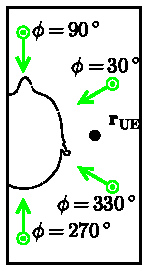
\includegraphics[width=0.885in]{figures/auto_induced_topview.pdf}};
        \end{tikzpicture}
        \caption{Auto-induced exposure setup. \Gls{MRT} beamforming aligns a number of plane waves (arrows) to focus at the \gls{UE} location. Each wave has a complex weight $w_i$ that can come from any direction. The inset shows our choice of directions. Phases align field contributions while amplitudes remain equal.}
        \label{fig:auto-ind}
    \end{subfigure}
\end{adjustwidth}
\centering
\caption{Exposure scenarios. (a)~Environmental exposure from 12 isotropic directions. (b)~Auto-induced exposure with beamforming from 4 directions.}
\label{fig:exposure-scenarios}
\end{figure*}

These 12 simulations can be combined to approximate exposure from arbitrary incident directions and polarizations.

\subsection{Auto-induced exposure scenario}
Figure~\ref{fig:exposure-scenarios}b shows the auto-induced exposure scenario with user-specific beamforming.
Auto-induced exposure occurs when a \gls{MaMIMO} base station beamforms toward a user's device, concentrating electromagnetic energy in a localized hotspot near the body.
Unlike environmental exposure, the incident field exhibits constructive interference at a focal point determined by the beamforming algorithm.
5G NR and anticipated 6G systems use user-specific beamforming to maximize link quality.

Previous work coupled \gls{MaMIMO} beamforming with site-specific propagation environments.
Hybrid ray-tracing and \gls{FDTD} methods enable realistic exposure assessment for indoor~\citep{shikhantsov2020massive,wydaeghe2022realistic} and outdoor~\citep{wydaeghe2025outdoor} scenarios, including stochastic channel models capturing real propagation statistics.
These studies show that exposure depends on environment, user position, and channel realization.
We take a different approach: rather than modeling specific environments and aggregating across channel realizations, we seek exposure estimates comparable across phantoms and frequencies without statistical bootstrapping~\citep{vermeeren2008sar,wydaeghe2022realistic}.

To simulate this auto-induced exposure scenario, plane waves were launched from four azimuthal directions ($\phi = 270\degree, 330\degree, 30\degree, 90\degree$) at a fixed co-elevation ($\theta = 90\degree$), representing a half-space illumination from the phantom's right side.
We chose $\theta = 90\degree$ (horizontal incidence) because base stations are typically mounted at or above head height, making horizontal incidence common, and this geometry maximizes the vertical electric field component $E_z$.
Only $\theta$ polarization was considered, as it produces the dominant vertical field component relevant for handheld device coupling \citep{shikhantsov2020massive}.

\subsubsection{Beamforming weights}
In \gls{MaMIMO} systems, \gls{MRT} is a common precoding technique that causes beamforming \citep{bjornson2017massive}.
For a channel vector $\mathbf{h} \in \mathbb{C}^N$ representing the complex gains from $N$ transmit directions to the \gls{UE}, the \gls{MRT} precoding vector (Frobenius-normalized) is
\begin{equation}
\mathbf{w} = \frac{\mathbf{h}^*}{\|\mathbf{h}\|} \,,
\label{eq:mrt_weights}
\end{equation}
which maximizes the received signal power $|y|^2 = |\mathbf{h}^\mathsf{T} \mathbf{w}|^2$~\citep{bjornson2017massive}.
Writing each channel element in polar form, $h_i = |h_i| \exp(j\phi_i)$, the weight becomes
\begin{equation}
w_i = \frac{|h_i|}{\|\mathbf{h}\|} \exp(-j\phi_i) \,.
\label{eq:mrt_polar}
\end{equation}
The phase term $\exp(-j\phi_i)$ conjugates the channel phase so that all contributions arrive in-phase at the receiver. This is the mechanism that produces constructive interference.
The amplitude term $|h_i|/\|\mathbf{h}\|$ allocates more power to directions with stronger channel gains.

In our framework, we interpret each channel $h_i$ as proportional to the vertical electric field component at the \gls{UE} location due to the $i$-th incident direction: $h_i \propto E_{z,i}(\mathbf{r}_0)$.
We assume the \gls{UE} antenna is vertically polarized, as is typical for handheld devices.
Because each $h_i$ is a per-direction channel in the angular domain rather than a per-antenna channel, this is a beamspace formulation of \gls{MRT} precoding.
The amplitude weighting in~\eqref{eq:mrt_polar} would require knowledge of which directions have stronger channels, information that depends on the propagation environment.

When simulating many environments using deterministic or stochastic channel models (e.g., ray-tracing or QuaDRiGa~\citep{wydaeghe2025outdoor}) and averaging the resulting exposure over all channel realizations, no single azimuthal direction consistently dominates.
All amplitudes are therefore set to $|w_i| = 1/\sqrt{N}$, yielding
\begin{equation}
w_i = \frac{1}{\sqrt{N}} \exp\bigl(-j\arg(E_{z,i}(\mathbf{r}_0))\bigr) \,.
\label{eq:equal_gain_weights}
\end{equation}
With this choice, $\|\mathbf{w}\|^2 = 1$ (unit total power) while the phase conjugation of \gls{MRT} is retained.
The combined field at any point $\mathbf{r}$ is then
\begin{equation}
\mathbf{E}_\mathrm{combined}(\mathbf{r}) = \sum_{i=1}^{N} w_i \, \mathbf{E}_i(\mathbf{r}) \,.
\label{eq:field_combination}
\end{equation}
We assume perfect channel state information and independent control of each incident direction, such that Eq.~\eqref{eq:field_combination} provides an upper bound on the achievable field concentration for a given total transmitted power.

The superposition in Eq.~\eqref{eq:field_combination} is exact because the tissue is linear.
Each $\mathbf{E}_i$ is a full-wave \gls{FDTD} solution that already contains the scattering, diffraction, and penetration of wave~$i$ into tissue.
Therefore, the combined field is defined throughout the body, on the surface and in the interior.
psSAR$_{10\mathrm{g}}$ is then averaged over a 10~g cubic mass inside tissue (IEC/IEEE~62704-1), and \gls{APD} over a 4~cm$^2$ skin-surface area (IEC/IEEE~63195-4).
The $N$ components together carry the incident power density of one plane wave.
The \gls{ICNIRP} reference level therefore applies directly.
Detailed hotspot field maps are reported in \citet{herssens2025autoinduced} and \citet{shikhantsov2020massive} for the same precoding family and phantoms.

Four azimuthal directions balance representativeness against computational cost.
In multipath propagation, effective channel rank is limited: singular value decomposition shows that a few principal components capture most channel energy~\citep{bjornson2017massive,wydaeghe2022realistic}.
Four directions spanning the azimuthal half-space capture the dominant modes of typical non-line-of-sight channels while keeping \gls{FDTD} simulations manageable.

\subsubsection{Focus point search}
\begin{figure}[!t]
    \centering
    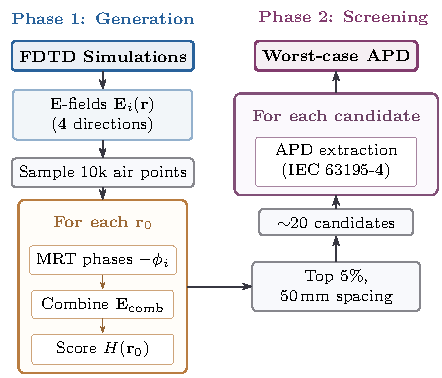
\includegraphics[width=3.5in]{figures/hotspot_score_flowchart.pdf}
    \caption{Two-stage screening reduces computational cost 500~times. Phase~1 evaluates 10,000 candidates using an efficient hotspot score based on E-field intensity at nearby skin voxels. Phase~2 performs full APD extraction following IEC/IEEE~63195-4 only on the top 20 candidates.}
    \label{fig:hotspot_flowchart}
\end{figure}
Figure~\ref{fig:hotspot_flowchart} summarizes the worst-case APD search procedure.
A \gls{MaMIMO} base station beamforms toward the \gls{UE} antenna, held in hand or pocket, always in air, at some distance from skin.
Therefore, the beamforming focus point lies in the air near the body surface, not inside the body.
The beam converges at this air location and illuminates nearby skin, where absorption occurs.

The search space comprises air voxels within a 20~mm shell surrounding the phantom surface.
This thickness covers realistic \gls{UE}-to-body distances while excluding voxels too far to produce substantial skin exposure.
From this space, 10,000 candidate focus points were randomly sampled, yielding approximately 10~mm average spacing given the 1.8~m$^2$ skin surface area of an adult phantom.

For FR3 simulations computing only APD, additional padding of 20~mm ($x$-direction) and 10~mm ($y$-direction) was added to accommodate focus points behind the phantom (e.g., near back or arms).
At FR1 frequencies (700~MHz and 3500~MHz), the search shell was widened to 50~mm (from 20~mm at FR3).
At sub-GHz wavelengths, a beam focused further from the surface still produces a meaningful hotspot on the skin.
The minimum candidate separation was increased to 100~mm, consistent with the 20$\times$ longer wavelength at 700~MHz ($\lambda = 430$~mm) compared to FR3.
The candidate pool was doubled to 40 per phantom with a lower selection percentile (80\% versus 95\% at FR3), because proxy correlation is weaker at these frequencies (see Section~\ref{sec:results_fr1_auto}).
At 3500~MHz and at FR3 frequencies, field combination was restricted to a 50~mm cube around each focus voxel.
The SAR peak at these frequencies occurs within millimetres of the focus on the skin surface.
At 700~MHz, SAR peaks can appear far from the focus point (see Section~\ref{sec:results_fr1_auto}), so full-volume combination over the entire body was used instead.

\subsubsection{Hotspot score for efficient worst-case identification}
\label{sec:hotspot_score}
Identifying the worst-case focus point requires evaluating APD for each candidate location.
Full APD extraction following IEC/IEEE~63195-4~\citep{iec63195} is computationally expensive: surface integration over 4~cm$^2$ averaging areas across the entire phantom surface.


We developed the \emph{hotspot score} that approximates APD without full extraction, exploiting the relationship between electric field intensity and \gls{APD}.
For a given air focus point $\mathbf{r}_0$, the hotspot score is defined as:
\begin{equation}
H(\mathbf{r}_0) = \frac{1}{N_\mathrm{skin}} \sum_{k=1}^{N_\mathrm{skin}} \bigl|\mathbf{E}_\mathrm{combined}(\mathbf{r}_k)\bigr|^2 \,,
\label{eq:hotspot_score}
\end{equation}
where the sum is over all $N_\mathrm{skin}$ skin voxels within a 50~mm cube centered on $\mathbf{r}_0$, and $\mathbf{E}_\mathrm{combined}$ is the weighted field from Eq.~\eqref{eq:field_combination} with weights computed for focus point $\mathbf{r}_0$ via Eq.~\eqref{eq:equal_gain_weights}.

The hotspot score works because APD $\propto \sigma |\mathbf{E}|^2$, where $\sigma$ is the tissue conductivity. Computing the hotspot score requires only reading pre-computed E-field values at skin voxel locations and performing the weighted combination. No additional \gls{FDTD} simulations or surface integrations are needed.
This enables rapid evaluation of all 10,000 candidate focus points. Candidates in the top 5\% by hotspot score were retained for full APD extraction.
To avoid clustering, a minimum separation of 50~mm was enforced: candidates were selected greedily in descending hotspot score order, skipping any candidate within 50~mm of an already-selected point.

\subsection{Numerical simulation framework}
We performed all simulations using Sim4Life 8.2~\citep{sim4life}, a GPU-accelerated \gls{FDTD} solver based on the Yee algorithm~\citep{yee1966numerical,taflove2005computational}.
\Gls{UPML} with 7 absorbing layers terminated the computational domain.
The \gls{TF/SF} formulation~\citep{taflove2005computational} realized far-field illumination.
All sources were harmonic excitations at frequencies listed in Table~\ref{table:simulation_parameters}, with 1~V/m incident amplitude.
Simulation duration was three times the domain diagonal traversal time in free space (6 cycles at 450~MHz, 500 cycles at 26~GHz).

Given the study scale (550 simulations across 15 frequencies, 4 phantoms, multiple directions and polarizations), we developed an open-source Python framework automating the simulation workflow.
Each simulation is defined by a JSON configuration file for reproducibility.

\subsection{Computational methodology}
Spatial discretization used a frequency-dependent scheme: 2.5~mm cells at 450--1450~MHz (10--32~\gls{CPW} in vitreous humor), reducing to 1.0--1.7~mm at 2140--5800~MHz, and 0.3--0.6~mm at FR3 frequencies.
Time stepping followed the \gls{CFL} stability limit~\citep{courant1928} ($\Delta t = \Delta x_\mathrm{min} / (c_0 \sqrt{3})$), yielding 4.81~ps at 450~MHz to 0.58~ps at 26~GHz.
Grid resolution was chosen to balance numerical accuracy (targeting 10~\gls{CPW} in high-permittivity tissues), skin mesh perforation (minimized at $\Delta x \leq 1.5$~mm), and computational cost (scaling with the fourth power of cell size without domain reduction).
The 90\% power absorption depth ($\delta_{90}$) decreases from $\sim$60~mm in muscle at 450~MHz to 1.1~mm in skin at 26~GHz, justifying coarser grids at low frequencies where penetration is deep. At sub-6~GHz frequencies, the absorption is not confined to the skin layer alone.
Complete details on discretization strategy, perforation analysis, and $\delta_{90}$ calculation are provided in the Supplementary Information.

\subsection{Anatomical phantoms}

We used four anatomically realistic human body models from the \gls{ViP} of the IT'IS Foundation~\citep{gosselin2014development}: two adults and two children, one for each sex.
The \gls{ViP} models (version 3.1) have 500~$\mu$m isotropic native resolution throughout the body.
Duke (adult male, 34y) and Ella (adult female, 26y) represent adults. Thelonious (male, 6y) and Eartha (female, 8y) represent children.
Each phantom comprises over 300 anatomical structures with tissue-specific dielectric properties.
Frequency-dependent dielectric properties ($\varepsilon_r$, $\sigma$) and mass density values came from the IT'IS tissue properties database (version~5)~\citep{itis_database}.


In addition to whole-body and peak spatial-average \gls{SAR}, regional \gls{SAR} was computed for four anatomical groups relevant to \gls{RF} exposure assessment: the brain, eyes, skin, and genitals.
These regions appear frequently in epidemiological studies and regulatory discussions.
Regional \gls{SAR} is defined as the mass-weighted average of \gls{SAR} values across all tissues in the group.
The \emph{brain group} comprises gray matter, white matter, cerebellum, hippocampus, thalamus, hypothalamus, midbrain, pons, medulla oblongata, hypophysis, pineal body, commissura anterior, commissura posterior, and cerebrospinal fluid.
The \emph{eyes group} comprises the cornea, lens, sclera, and vitreous humor.
The \emph{skin group} comprises, as defined by Sim4Life, the skin and ``Ear skin'' entities.
The \emph{genitals group} comprises sex-specific reproductive organs. For male phantoms (Duke, Thelonious) it includes testis, epididymis, prostate, and penis. For female phantoms (Ella, Eartha) it includes ovary, uterus, and vagina.


\subsection{Computational efficiency strategies}
At FR3 and FR2 frequencies, fine grid resolution produces computational domains with hundreds of millions to billions of cells.
Two domain reduction strategies and cloud infrastructure made these simulations tractable.

\subsubsection{Half-body symmetry}
For incidence directions illuminating only one side of the body (e.g., $+x$ illuminating the right side), the domain was truncated to include only the illuminated half.
The boundary was placed at the sagittal midplane with \gls{PML} termination.
This works because high-frequency penetration depth is small enough that fields on the illuminated side do not couple to the opposite side.
The ``$x$/2'' notation in Table~\ref{table:simulation_parameters} indicates this reduction.
Tissues that straddle the midplane sit against this boundary, so their metrics are excluded where the reduction is used (Section~\ref{sec:results_crossband}).

\subsubsection{Height factor reduction}
Above 7~GHz, domain height was further reduced by a frequency-dependent height factor $h$.
We chose 7~GHz as the reference because at this frequency the domain reaches approximately 800~million cells for adult phantoms, a practical limit beyond which GPUs struggle with memory even in multi-GPU configurations.
The height reduction starts by removing the lower body (feet and legs), as peak absorption in the auto-induced scenario occurs in the head and upper torso region.

The height factor was computed as:
\begin{equation}
h = \left(\frac{\Delta x_f}{\Delta x_{7\,\mathrm{GHz}}}\right)^3 \,,
\end{equation}
where $\Delta x_f$ is the cell size at frequency $f$ and $\Delta x_{7\,\mathrm{GHz}} = 0.6$~mm is the reference cell size at 7~GHz.
This cubic scaling keeps the number of grid cells roughly constant as frequency increases: the cell counts for Duke, Ella, Eartha, and Thelonious remain within 2\% of their 7~GHz values across the entire FR3 band (Table~\ref{table:simulation_parameters}).
At 15~GHz, for example, $h = (0.4/0.6)^3 \approx 0.30$, meaning only the top 30\% of the phantom height is simulated.

We validated this reduction against full-body simulations (Supplementary Information).
At~3.5~GHz, removing the lower~70\% of the body ($h=0.30$) changes the local peak metrics, psSAR$_{10\mathrm{g}}$ and head-organ \gls{SAR}, by less than~4\%.
The reduction is applied only above~7~GHz, where the penetration depth is shorter and the error smaller.
The same sweep at~450~MHz moves the metrics by up to~53\%, which is why the full body is retained at all frequencies $\le 7$~GHz.

Without this height reduction, simulations at 15~GHz would require approximately 2.8~billion cells per phantom, over three times the 7~GHz baseline.
The time step also decreases with frequency (from 1.16~ps at 7~GHz to 0.77~ps at 15~GHz), adding to the computational cost.
For the 26~GHz simulation, the height factor approach was not applied ($h = 1$) to compute SAR$_\mathrm{wb}$.
Instead, only the smallest phantom (Thelonious) was simulated from a single incidence direction, using half-body symmetry reduction.
The same single-direction approach was used for Thelonious at FR3 frequencies to allow \gls{SAR} extraction for comparison with APD (``Half (for SAR)'' entries in Table~\ref{table:simulation_parameters}).
Even with these simplifications, the 26~GHz simulation required 1.84~billion cells and multiple 48~GB GPUs.

\subsubsection{Computational resources and campaign scale}
We executed simulations on rented cloud GPU instances (TensorDock) with NVIDIA H100, RTX~5090, and RTX~6000 GPUs, sometimes in multi-GPU workstations, paired with 32--256~GB RAM.
Cloud infrastructure was chosen over traditional \gls{HPC} because our \gls{HPC} options impose quotas and queues, and Sim4Life requires Windows with licensing better suited to workstations.

The campaign comprised 550 individual \gls{FDTD} runs across all phantom-frequency-direction-polarization combinations.
Simulations ranged from 11 million cells (Thelonious at 450~MHz) to 1.84 billion cells (Thelonious at 26~GHz).
Computational cost varied considerably due to $f^4$ scaling. Duke at 450~MHz completes in under 5 minutes, at 5.8~GHz in 25 minutes, and at 26~GHz (Thelonious only, half-body) in over 2 hours, at which point I/O-bound setup and extraction phases took similar time.

\section{Results}
\label{sec:results}

The simulations produced a large multi-dimensional dataset.
This section summarizes the main findings.
Supplementary Information contains more data: per-tissue \gls{SAR} values for each frequency and direction, frequency response curves for individual organs, spatial hotspot maps, and cross-phantom comparisons.

For comparison with \gls{ICNIRP} basic restrictions for general public exposure, the limits are 0.08~W/kg for whole-body average \gls{SAR}, 2~W/kg for local psSAR$_{10\mathrm{g}}$ (head and trunk), and 20~W/m$^2$ for APD above 6~GHz (Table~\ref{table:icnirp_limits}).

\subsection{FR1 environmental exposure}
\label{sec:results_fr1_env}

All \gls{SAR} values in this section are normalized to an incident power density of 1~W/m$^2$.
The \gls{ICNIRP} 2020 reference levels for general public exposure are $S_\mathrm{ref} = f_\mathrm{MHz}/200$~W/m$^2$ for frequencies below 2~GHz, and 10~W/m$^2$ at 2~GHz and above.
SAR values can be scaled by these factors to obtain values at the reference level.

\subsubsection{Penetration depth determines the frequency response}

Figure~\ref{fig:sar_divergence} shows the normalized \gls{SAR} as a function of frequency.
The 90\% power absorption depth ($\delta_{90}$) on the body decreases from $\sim$60~mm at 450~MHz to $\sim$10~mm at 5800~MHz.
This shift from volumetric to superficial absorption drives all \gls{SAR} metrics.

Figure~\ref{fig:sar_divergence} shows opposite trends for different tissue groups.
Skin \gls{SAR} increases by a factor 3.2 between 450~MHz and 5800~MHz, as energy concentrates superficially.
Brain \gls{SAR} decreases by 96\% between 450~MHz and 5800~MHz, because skull and overlying tissues absorb most energy before it reaches the brain.
Whole-body \gls{SAR} decreases by a factor 2.1 between 450~MHz and 5800~MHz, because total absorbed power decreases when absorption confines to a thin surface layer.

\begin{figure}[!t]
    \centering
    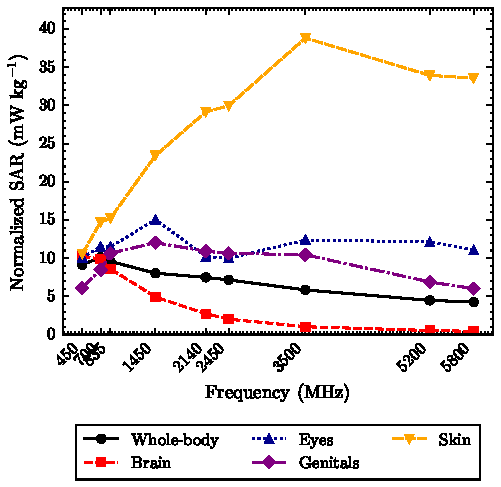
\includegraphics[width=3.5in]{figures/sar_divergence.pdf}
    \caption{Skin \gls{SAR} increases 3.2~times while brain \gls{SAR} decreases 96\% across FR1. Mass-averaged \gls{SAR} by tissue group for Thelonious, averaged across all 12 directions and polarizations. Eyes show a non-monotonic response.}
    \label{fig:sar_divergence}
\end{figure}

Figure~\ref{fig:penetration_ratio} shows the transition in the brain-to-skin \gls{SAR} ratio across all phantoms.
At 450~MHz, the ratio ranges from 0.74 to 1.05, meaning brain and skin \gls{SAR} are comparable.
As frequency increases, the ratio drops significantly for all phantoms.
At 5800~MHz, the ratios decrease to between 0.003 and 0.015.
Child phantoms maintain higher relative penetration at high frequencies compared to adults.
This two-order-of-magnitude decrease across the FR1 band shows the shift from penetrating to superficial absorption.

\begin{figure}[!t]
    \centering
    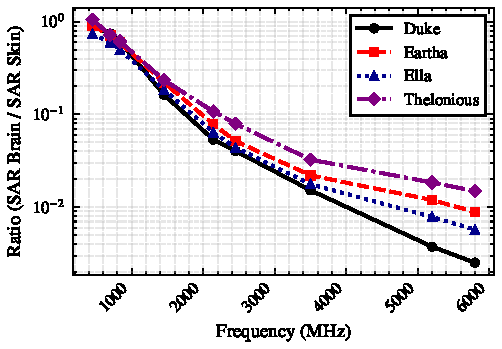
\includegraphics[width=3.5in]{figures/penetration_ratio.pdf}
    \caption{Brain-to-skin \gls{SAR} ratio across phantoms. Brain exposure drops by orders of magnitude relative to skin as frequency increases. Child phantoms show higher relative brain exposure at high frequencies compared to adults.}
    \label{fig:penetration_ratio}
\end{figure}

\subsubsection{Tissue-specific absorption}

Figure~\ref{fig:tissue_ranking} ranks the 20 tissues with highest mass-averaged \gls{SAR}, averaged across all frequencies and directions.
Ear cartilage (36.9~mW/kg) and ear skin (29.5~mW/kg) absorb significantly more power per unit mass than bulk skin (21.5~mW/kg).
Their peripheral position and thin geometry explain this: the pinna is exposed from multiple directions and lacks underlying tissue to absorb incident energy.

\begin{figure}[!t]
    \centering
    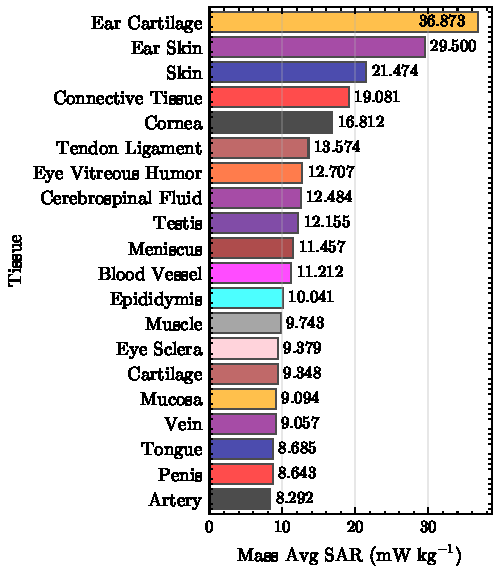
\includegraphics[width=3.5in]{figures/tissue_ranking.pdf}
    \caption{Ear tissues absorb twice as much power per unit mass as bulk skin. Top 20 tissues ranked by mass-averaged \gls{SAR} for Thelonious, averaged across all frequencies in FR1 and directions. Cornea, testis, and meniscus also rank in the top 10.}
    \label{fig:tissue_ranking}
\end{figure}

Cornea ranks fifth (16.8~mW/kg), consistent with the eye's exposed position.
Testis ranks ninth (12.2~mW/kg), receiving substantial frontal exposure despite pelvic shielding from other angles.
Meniscus ranks tenth (11.5~mW/kg).
Inside the skull, \gls{CSF} ranks eighth (12.5~mW/kg), higher than gray matter (5.6~mW/kg) and white matter (3.2~mW/kg), due to its high water content and conductivity.

For psSAR$_{10\mathrm{g}}$, the 10~g averaging volume smooths tissue-specific variations.
Skin dominates (83.5~mW/kg), followed by subcutaneous fat (81.4~mW/kg), muscle (75.7~mW/kg), and bone (73.7~mW/kg).
Small tissues like ear cartilage (7~g total mass) cannot fill a 10~g cube and thus do not appear in the psSAR$_{10\mathrm{g}}$ ranking.

\subsubsection{Children have higher whole-body \gls{SAR} than adults}

Figure~\ref{fig:cross_phantom} compares whole-body \gls{SAR} across phantoms.
Child phantoms (Thelonious, 6y, and Eartha, 8y) show 1.5--1.9~times higher SAR$_\mathrm{wb}$ than adults (Duke, Ella) at all frequencies.
At 700~MHz, Thelonious reaches 10.1~mW/kg versus Duke's 5.5~mW/kg (ratio 1.85).

\begin{figure}[!t]
    \centering
    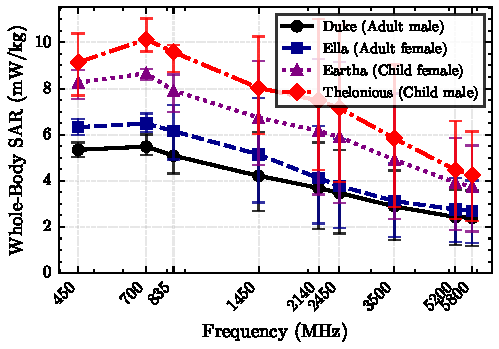
\includegraphics[width=3.5in]{figures/cross_phantom_sar_wb.pdf}
    \caption{Children show 1.5--1.9~times higher whole-body \gls{SAR} than adults at all frequencies. Error bars indicate standard deviation across the 12 direction-polarization combinations.}
    \label{fig:cross_phantom}
\end{figure}

The higher whole-body \gls{SAR} in children follows from the relationship between \gls{SAR}, absorption cross section (ACS), and body mass~\citep{bamba2015absorption}:
\begin{equation}
\mathrm{SAR}_\mathrm{wb} = \frac{\mathrm{ACS}_\mathrm{wb} \times S}{m}
\label{eq:sar_acs}
\end{equation}
where $\mathrm{ACS}_\mathrm{wb}$ is the whole-body absorption cross section (in m$^2$), $S$ is the incident power density, and $m$ is body mass.
Although children have smaller $\mathrm{ACS}_\mathrm{wb}$ than adults (less body surface area), their mass is proportionally much smaller.
The ratio $\mathrm{ACS}_\mathrm{wb}/m$ is approximately 50\% higher in a 6-year-old than in an adult, meaning children absorb more power per kilogram of body mass.
At sub-GHz frequencies, body dimensions approach fractions of the wavelength ($\lambda = 43$~cm at 700~MHz), potentially producing quasi-resonance effects that differ between body sizes.

\subsubsection{Direction and polarization dependence}

Table~\ref{table:direction_var} summarizes directional variation for each \gls{SAR} metric (Thelonious, frequency-averaged values).
Similar patterns are observed for the other phantoms: frequency-averaged whole-body \gls{SAR} varies 2.0--2.3$\times$ across phantoms, skin 4.5--6.4$\times$, eyes 20--36$\times$, and brain 3.6--6.0$\times$ (all phantoms, see Tables S3--S6 in the Supplementary Information).
Genitals show the largest inter-phantom difference in directional variation, ranging from 9--10$\times$ for females (Ella, Eartha) to 46--67$\times$ for males (Duke, Thelonious).
For Thelonious, eyes show 20-fold variation: frontal exposure yields 28.9~mW/kg versus 1.4~mW/kg from behind, as the cornea is exposed while the skull shields posteriorly.
Genitals show 44-fold variation between frontal and below directions. The body shields the pelvic region from most angles.
Brain shows only 4-fold variation: the skull shields from all directions.
Whole-body \gls{SAR} varies 2-fold.

\begin{table}[!t]
\centering
\caption{Directional Variation in \gls{SAR} Metrics (Thelonious, frequency-averaged values).}
\label{table:direction_var}
\begin{tabular}{@{}lccc@{}}
\toprule
\textbf{Metric} & \textbf{Max} & \textbf{Min} & \textbf{Max/Min} \\
 & \textbf{(mW/kg)} & \textbf{(mW/kg)} & \\
\midrule
Eyes SAR & 28.9 (front) & 1.4 (back) & 20$\times$ \\
Genitals SAR & 30.5 (front) & 0.7 (below) & 44$\times$ \\
Brain SAR & 6.5 (below) & 1.8 (above) & 4$\times$ \\
Skin SAR & 41.3 (front) & 9.2 (above) & 4$\times$ \\
Whole-body SAR & 10.3 (back) & 5.3 (below) & 2$\times$ \\
\bottomrule
\end{tabular}
\end{table}

Polarization generally has smaller effect than direction.
Figure~\ref{fig:polarization_ratio} shows the polarization ratio for different tissue groups and incident directions.
The $\theta$/$\phi$ polarization ratio ranges from 0.8 to 1.6 for skin and whole-body \gls{SAR}.
Genitals are an exception. From below, the ratio reaches 1.8, indicating stronger coupling to vertically polarized fields. From above, it drops to 0.12.
The results may be underestimated because material properties from the IT'IS database are isotropic.

The IT'IS database also assigns age-independent dielectric properties.
The child phantoms therefore have child anatomy but adult tissue properties.
Age-independent properties are standard in numerical dosimetry~\citep{bakker2010children,kuehn2009assessment,gosselin2014development}.
A closed-form Fresnel analysis shifts the \gls{APD} and whole-body \gls{SAR} conservatively, by~6--10\%.
This shift is comparable to the~4--9\% that a~10--20\% dielectric-parameter uncertainty propagates onto the same metrics.
Our compliance conclusions are therefore robust to a shift of this size, and the Supplementary Information reports the full analysis.

We collect these effects into one uncertainty budget (Supplementary Information).
The dominant random contributions are the tissue-dielectric spread and the \gls{FDTD} numerical error.
Combined in quadrature, they give an expanded uncertainty of about~$\pm 12\%$ on the absorbed-power metrics, at a 95\% coverage probability.
The age and domain-truncation effects act in one direction, conservatively.

\begin{figure}[!t]
    \centering
    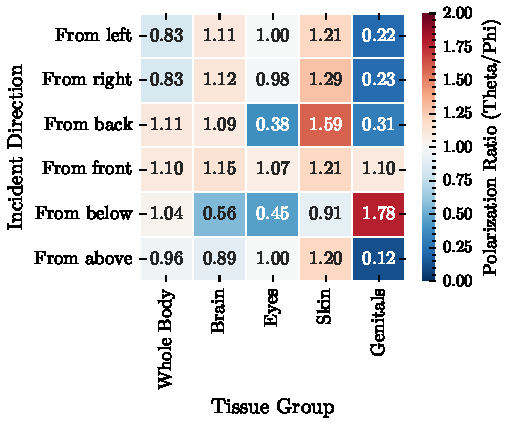
\includegraphics[width=3.5in]{figures/polarization_ratio.pdf}
    \caption{Polarization ratio ($\theta/\phi$) for different tissue groups and incident directions. Values near 1 indicate insensitivity. Genitals show strong polarization sensitivity (ratio = 1.8 from below). Whole-body \gls{SAR} remains insensitive.}
    \label{fig:polarization_ratio}
\end{figure}

\subsubsection{Correlation between \gls{SAR} metrics}

The correlation matrix across all 432 simulation configurations shows that most metrics are independent, with one protective effect.
Skin \gls{SAR} and brain \gls{SAR} correlate negatively ($r = -0.45$, $p < 0.001$): high skin absorption reduces energy available for deeper penetration.
Superficial absorption shields deep tissues.

Whole-body \gls{SAR} and skin \gls{SAR} are nearly uncorrelated ($r = -0.04$).
At low frequencies, deep tissues (muscle, organs) dominate whole-body \gls{SAR}. At high frequencies, whole-body \gls{SAR} decreases even as the skin fraction increases.
These opposing trends cancel.

psSAR$_{10\mathrm{g}}$ values for different organs are largely independent. Skin and genitals correlate at only $r = 0.14$. Brain and eyes correlate at $r = 0.54$ (both head-region metrics).
Worst-case exposure for one organ does not predict worst-case for others.

\subsubsection{Compliance margins at reference levels}
\label{sec:compliance_fr1}

Table~\ref{table:compliance_fr1} compares direction-averaged \gls{SAR} at the \gls{ICNIRP} reference levels against the basic restrictions.
The reference level $S_\mathrm{ref}$ increases from 2.25~W/m$^2$ at 450~MHz to 10~W/m$^2$ at 2~GHz and above.
The rightmost column shows the percentage of the basic restriction reached by the maximum \gls{SAR} value across all four phantoms.

\begin{table}[!t]
\centering
\caption{Direction-Averaged Whole-Body SAR at ICNIRP Reference Levels (FR1).}
\label{table:compliance_fr1}
\begin{tabular}{@{}lccccccc@{}}
\toprule
\textbf{Freq} & \textbf{$S_\mathrm{ref}$} & \textbf{Duke} & \textbf{Ella} & \textbf{Eartha} & \textbf{Thelonious} & \textbf{\% of limit$^a$} \\
\textbf{(MHz)} & \textbf{(W/m$^2$)} & \textbf{(M,34y)} & \textbf{(F,26y)} & \textbf{(F,8y)} & \textbf{(M,6y)} & \\
\cmidrule(lr){3-6}
 & & \multicolumn{4}{c}{\textbf{Direction-averaged SAR$_\mathrm{wb}$ (mW/kg)}} & \\
\midrule
450 & 2.25 & 12.0 & 14.2 & 18.6 & 20.6 & 26\% \\
700 & 3.50 & 19.2 & 22.7 & 30.3 & 35.5 & 44\% \\
835 & 4.18 & 21.3 & 25.7 & 33.1 & 40.0 & 50\% \\
1450 & 7.25 & 30.5 & 37.3 & 48.9 & 58.2 & 73\% \\
2140 & 10.0 & 36.9 & 41.2 & 61.6 & 74.8 & \textbf{93\%} \\
2450 & 10.0 & 34.7 & 37.8 & 59.0 & 71.5 & 89\% \\
3500 & 10.0 & 28.9 & 31.2 & 49.1 & 58.4 & 73\% \\
5200 & 10.0 & 24.3 & 27.6 & 39.3 & 44.7 & 56\% \\
5800 & 10.0 & 24.0 & 27.0 & 37.5 & 42.6 & 53\% \\
\bottomrule
\multicolumn{7}{@{}l}{\footnotesize $^a$Maximum across all four phantoms. Basic restriction SAR$_\mathrm{wb}$ = 80~mW/kg.}
\end{tabular}
\end{table}

Whole-body \gls{SAR} peaks near 2140~MHz for all phantoms, giving the tightest compliance margin in the FR1 band.
Thelonious reaches 93\% of the basic restriction at this frequency.
Child phantoms (Thelonious, Eartha) exceed adults by a factor of 1.7--1.9 across all frequencies.
Sex accounts for less than 20\% variation within each age group.
Adult phantoms remain below 52\% of the basic restriction at all frequencies.

These values are averaged over the 12 directions.
The worst single configuration (front or back incidence) is 1.5--1.6 times higher.
Under that configuration both child phantoms exceed the basic restriction near 2140~MHz.
Thelonious is at 145\% of the limit and Eartha at 122\%.
Four of the twelve configurations exceed the limit for each of them.
Duke and Ella are below 82\% in every configuration.

These values occur at the \gls{ICNIRP} reference level.
A ten-country measurement campaign found environmental power densities of 0.33--1.72~mW/m$^2$, three to four orders of magnitude below the 10~W/m$^2$ reference level~\citep{veludo2025assessing}.
At the highest measured level, the worst configuration for Thelonious is 4000 times below the basic restriction.

For psSAR$_{10\mathrm{g}}$, margins are substantially larger.
Skin psSAR$_{10\mathrm{g}}$ reaches 909~mW/kg at 2140~MHz for Duke at the reference level (45\% of the 2000~mW/kg limit).
Brain and eyes psSAR$_{10\mathrm{g}}$ reach 178~mW/kg and 137~mW/kg, respectively (9\% and 7\% of the limit).
These are direction-averaged values as well.
In the worst configuration, Eartha is at 129\% of the 2~W/kg head and torso restriction at 2140~MHz.
The peak is located in the hand, where the limb restriction of 4~W/kg applies instead.
Against that restriction, Eartha is at 65\%.
psSAR$_{10\mathrm{g}}$ is therefore below its applicable restriction in every environmental configuration.
Whole-body \gls{SAR}, not local \gls{SAR}, is the limiting metric for FR1 environmental exposure, for the direction average and for the worst case.

\subsection{SAR trends extended to FR3 and FR2}
\label{sec:results_crossband}

All \gls{SAR} values in this section are normalized to 1~W/m$^2$ incident and cover Thelonious (M, 6y) under right-side illumination ($\theta$ polarization) at 7--26~GHz.
Brain \gls{SAR} is excluded: structures at the sagittal cut face of the half-phantom show \gls{SAR} increasing with frequency, opposite to the physical expectation for deep tissue (PML boundary artifact).
Genitals \gls{SAR} is excluded by the same mechanism: the penis and prostate run along the sagittal midplane and are cut and exposed to the PML face.

\subsubsection{Skin and eye \gls{SAR} across the full band}

Figure~\ref{fig:sar_trends_fr1_to_fr2} shows skin \gls{SAR}, eye \gls{SAR}, and whole-body \gls{SAR} from 450~MHz to 26~GHz.
Skin \gls{SAR} continues to rise: 18.6~mW/kg at 5800~MHz (FR1, right-side), 21.5~mW/kg at 7~GHz, and 39.8~mW/kg at 26~GHz.
The $\delta_{90}$ on the body falls from $\sim$10~mm at 5800~MHz to 1.1~mm in skin at 26~GHz, concentrating absorption in a progressively thinner surface layer.

\begin{figure}[!t]
    \centering
    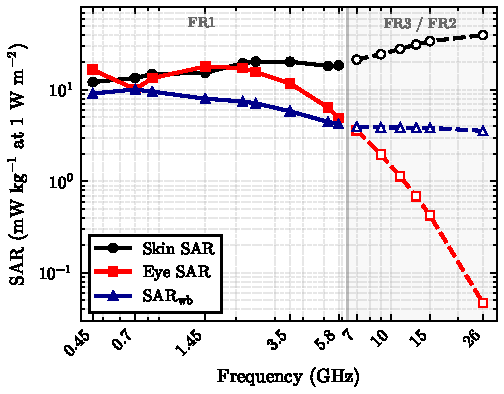
\includegraphics[width=3.5in]{figures/sar_trends_fr1_to_fr2.pdf}
    \caption{Eye \gls{SAR} collapses 77-fold from 7 to 26~GHz as penetration depth falls below eyelid thickness. Skin \gls{SAR} rises through the full band. Mass-averaged \gls{SAR} for Thelonious. Solid lines: FR1. Dashed lines: FR3 and FR2. Skin and eye \gls{SAR}: right-side illumination throughout. Whole-body \gls{SAR}: FR1 solid = 12-direction isotropic average, FR3/FR2 dashed = single right-side direction. Brain and genitals \gls{SAR} are excluded due to PML boundary artifacts in the FR3 half-phantom.}
    \label{fig:sar_trends_fr1_to_fr2}
\end{figure}

Eye \gls{SAR} falls from 4.92~mW/kg at 5800~MHz to 3.62~mW/kg at 7~GHz, then to 0.047~mW/kg at 26~GHz, a 77-fold decrease across FR3 and FR2.
The Thelonious phantom has closed eyes. The eyelid skin covers the cornea.
At 26~GHz, $\delta_{90}$ in skin falls to 1.1~mm, comparable to eyelid thickness, and incident energy is absorbed in the eyelid before reaching the cornea.
The FR1/FR3 boundary is smooth for both skin and eye \gls{SAR}.
Whole-body \gls{SAR} is normalized by the full-body mass.
The shadow half absorbs only the diffraction from the plane wave, limited at 7~GHz, so the illuminated half carries the body's absorbed power.
The value is 4.0~mW/kg at 7~GHz (single direction), continuous with the 4.3~mW/kg 12-direction average at 5800~MHz.
The whole-body \gls{SAR} stays flat near 3.6--4.0~mW/kg across FR3 and FR2.

\subsubsection{psSAR$_{10\mathrm{g}}$ continuation}

psSAR$_{10\mathrm{g}}$ connects smoothly at the band boundary: 63.5~mW/kg at 5800~MHz, 60.4~mW/kg at 7~GHz, and 50.3~mW/kg at 26~GHz.
The decrease is 21\% from 5800~MHz to 26~GHz.
Spatial averaging over 10~g smooths the increasingly confined surface absorption. As energy concentrates in a thinner layer, the peak spread over a fixed 10~g volume changes slowly.
The 12-direction isotropic psSAR$_{10\mathrm{g}}$ at 5800~MHz is approximately 116~mW/kg, roughly twice the single-direction value. FR3 and FR2 values likewise underestimate the isotropic worst case.

\subsection{FR1 auto-induced exposure}
\label{sec:results_fr1_auto}

All values are normalized to 1~W/m$^2$ incident and scale proportionally at the reference level ($S_\mathrm{ref} = 3.5$~W/m$^2$ at 700~MHz, 10~W/m$^2$ at 3500~MHz).
ICNIRP (2020) basic restrictions for local SAR are psSAR$_{10\mathrm{g}} = 2$~W/kg (head/torso) and 4~W/kg (limbs). For whole-body exposure, SAR$_\mathrm{wb} = 80$~mW/kg.

\subsubsection{psSAR$_{10\mathrm{g}}$ at 700~MHz and 3500~MHz}

Table~\ref{table:fr1_auto} compares auto-induced and environmental psSAR$_{10\mathrm{g}}$ and SAR$_\mathrm{wb}$ at both frequencies.
At 3500~MHz, auto-induced psSAR$_{10\mathrm{g}}$ exceeds the basic restriction for all four phantoms at the reference level.
Worst-case values reach 131--158\% of the 2~W/kg head/torso limit, with the SAR peak located in the torso, chest, or neck for all four phantoms.
At 700~MHz, all phantoms comply.
Duke and Eartha peak in the lower leg, where the 4~W/kg limb limit applies, reaching 22\% and 30\% respectively.
Ella and Thelonious peak in the torso (49\% and 48\% of the 2~W/kg limit).

For 3500~MHz, the environmental value for Thelonious already reaches 98\% of the basic restriction at $S_\mathrm{ref}$, and beamforming causes non-compliance for all four phantoms.
This scenario uses simplified \gls{MRT} beamforming from four directions and is not an upper bound.
Coherent array gain grows with the number of antenna elements~\citep{marzetta2016fundamentals}.
Richer propagation environments provide more multipath components for constructive interference, so higher local SAR values are physically feasible.
Real deployments vary beam direction with user movement and channel dynamics (e.g., with \gls{TDMA}), which reduces time-averaged exposure.

These values occur at the \gls{ICNIRP} reference level.
A ten-country measurement campaign found 2.61--11.12~mW/m$^2$ at 3500~MHz under continuous worst-case downloading, three orders of magnitude below that level~\citep{veludo2025assessing}.
Realistic exposure is well below the basic restrictions.

At 700~MHz, the environmental value is well within compliance, and beamforming roughly doubles psSAR$_{10\mathrm{g}}$ with ample margin to the limit.
The weak proxy correlation at 700~MHz (Section~\ref{sec:fr1_proxy}) means the reported values may not represent the absolute worst case across all possible focus points.
The margin to the local-SAR basic restriction (at most 49\% at $S_\mathrm{ref}$) is large enough that this uncertainty does not affect the compliance conclusion.

SAR$_\mathrm{wb}$ at 700~MHz is essentially unchanged by beamforming.
Auto-induced SAR$_\mathrm{wb}$ ranges 6.5--11.7~mW/kg across phantoms at 1~W/m$^2$, within the spread of environmental values (4.1--12.4~mW/kg across the 12 directions).
Coherent focusing redistributes absorption spatially without increasing total absorbed power.

\begin{table}[!t]
\centering
\caption{Auto-induced psSAR$_{10\mathrm{g}}$ and SAR$_\mathrm{wb}$ compared to the environmental worst case. All values at 1~W/m$^2$ incident. The \% limit column gives psSAR$_{10\mathrm{g}}$ as a percentage of the applicable local-SAR basic restriction at $S_\mathrm{ref}$.}
\label{table:fr1_auto}
\begin{tabular}{@{}l cc cc c cc c@{}}
\toprule
& \multicolumn{5}{c}{\textbf{700~MHz} ($S_\mathrm{ref} = 3.5$~W/m$^2$)} & \multicolumn{3}{c}{\textbf{3500~MHz} ($S_\mathrm{ref} = 10$~W/m$^2$)} \\
\cmidrule(lr){2-6} \cmidrule(lr){7-9}
& \multicolumn{2}{c}{psSAR$_{10\mathrm{g}}$} & \multicolumn{2}{c}{SAR$_\mathrm{wb}$} & & \multicolumn{2}{c}{psSAR$_{10\mathrm{g}}$} & \\
& \multicolumn{2}{c}{[mW/kg]} & \multicolumn{2}{c}{[mW/kg]} & \% limit & \multicolumn{2}{c}{[mW/kg]} & \% limit \\
Phantom & Env. & Auto. & Env. & Auto. & at $S_\mathrm{ref}$ & Env. & Auto. & at $S_\mathrm{ref}$ \\
\midrule
Duke (M, 34y)      & 129 & 253 &  6.7 &  6.5 & 22\%$^a$ & 156 & 266 & 133\%$^b$ \\
Eartha (F, 8y)     & 173 & 339 & 11.2 & 11.6 & 30\%$^a$ & 159 & 305 & 152\%$^b$ \\
Ella (F, 26y)      & 168 & 280 &  8.3 &  7.5 & 49\%     & 135 & 316 & 158\%$^b$ \\
Thelonious (M, 6y) & 132 & 275 & 12.4 & 11.7 & 48\%     & 197 & 262 & 131\%$^b$ \\
\bottomrule
\multicolumn{9}{@{}l}{\footnotesize $^a$Peak in lower leg. Limb limit (4~W/kg) applies.} \\
\multicolumn{9}{@{}l}{\footnotesize $^b$Peak in torso/chest/neck. Head/torso limit (2~W/kg) applies.} \\
\multicolumn{9}{@{}l}{\footnotesize \phantom{$^b$}See supplementary information for body-height distributions.}
\end{tabular}
\end{table}

\subsubsection{Proxy reliability and candidate search}
\label{sec:fr1_proxy}

The hotspot-score proxy that reliably identifies worst-case APD at FR3 performs differently across the two FR1 frequencies.
At 3500~MHz, Spearman rank correlation between proxy score and psSAR$_{10\mathrm{g}}$ ranges from $\rho = 0.70$ to $0.80$ ($p < 0.001$) across phantoms.
The worst-case candidate ranks within the top~8 for all phantoms (top~2 for Duke and Ella, top~1 for Thelonious).

At 700~MHz, rank correlation drops to $\rho = 0.27$--$0.42$.
Duke's worst case ranks 36th of 40 by proxy score.
At this frequency ($\lambda = 430$~mm), body dimensions approach resonance, diffraction wraps fields around the body, and the SAR peak location decouples from the beam focus point.
Duke illustrates the effect: the focus voxel lies in the head region, yet the SAR peak occurs in the lower leg (10\% of body height).
The proxy predicts near-surface field concentration but not deep-tissue absorption at sub-GHz wavelengths (see supplementary material for focus-$z$ vs.\ peak-$z$ scatter plots).
A larger candidate pool of 40 per phantom compensated for the proxy's weak discriminating power at 700~MHz.

\subsection{FR3 auto-induced exposure}
\label{sec:results_fr3_auto}

All APD values in this section are normalized to an incident power density of 1~W/m$^2$.
At the \gls{ICNIRP} reference level of 10~W/m$^2$ (applicable above 2~GHz), values scale by a factor of 10.
The basic restriction is APD $= 20$~W/m$^2$ averaged over 4~cm$^2$.

\subsubsection{ICNIRP limit exceeded at 7~GHz}

Figure~\ref{fig:fr3_compliance} shows each phantom's APD as a percentage of the basic restriction across the FR3 band.
Thelonious (6y) reaches 103\% of the basic restriction at 7~GHz, the only configuration exceeding the \gls{ICNIRP} limit.
Worst-case APD at the reference level is 20.5~W/m$^2$, exceeding the 20~W/m$^2$ limit by 2.5\%.
Previous studies have reported exceedances of basic restrictions when reference levels are met, particularly for small children at lower frequencies~\citep{vermeeren2008electronics}.

\begin{figure}[!t]
    \centering
    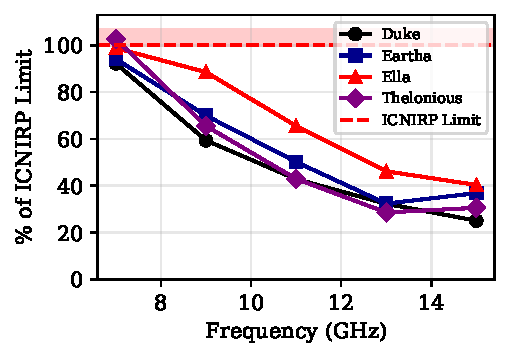
\includegraphics[width=3.5in]{figures/icnirp_compliance_by_frequency.pdf}
    \caption{Thelonious (6y) exceeds the ICNIRP basic restriction at 7~GHz (103\%). Percentage of the basic restriction versus frequency for auto-induced exposure at 10~W/m$^2$ reference level. Shaded region above 100\% indicates non-compliance. At 15~GHz, all phantoms fall below 40\%.}
    \label{fig:fr3_compliance}
\end{figure}

At 7~GHz, all phantoms reach 90\% or more of the basic restriction: Duke (92\%), Eartha (94\%), Ella (99\%), and Thelonious (103\%).
Compliance margins improve at higher frequencies: at 15~GHz, all phantoms fall below 40\% of the basic restriction.
The wavelength-to-averaging-area relationship explains this: at 7~GHz ($\lambda = 43$~mm), the \gls{MRT}-focused beam forms a hotspot comparable to the 4~cm$^2$ averaging area, maximizing averaged power density.
At 15~GHz ($\lambda = 20$~mm), the smaller hotspot size spreads power over less of the averaging region.

\subsubsection{Peak APD decreases with frequency}

Table~\ref{table:sapd_fr3} lists worst-case APD for each phantom-frequency combination.
Peak APD decreases 3--4$\times$ from 7~GHz to 15~GHz for all phantoms.
Thelonious shows the highest value at 7~GHz (2.05~W/m$^2$ at 1~W/m$^2$ incident). Duke shows the lowest (1.84~W/m$^2$).
The child-to-adult ratio is approximately 1.1 at 7~GHz, smaller than the 1.5--1.9 ratio for whole-body \gls{SAR} in FR1.

\begin{table}[!t]
\centering
\caption{Worst-Case APD by Phantom and Frequency (W/m$^2$ at 1~W/m$^2$ incident).}
\label{table:sapd_fr3}
\begin{tabular}{@{}lccccc@{}}
\toprule
\textbf{Phantom} & \textbf{7~GHz} & \textbf{9~GHz} & \textbf{11~GHz} & \textbf{13~GHz} & \textbf{15~GHz} \\
\midrule
Duke & 1.84 & 1.19 & 0.86 & 0.65 & 0.50 \\
Ella & 1.98 & 1.77 & 1.31 & 0.92 & 0.81 \\
Eartha & 1.88 & 1.40 & 1.00 & 0.65 & 0.74 \\
Thelonious & \textbf{2.05} & 1.31 & 0.86 & 0.57 & 0.61 \\
\bottomrule
\end{tabular}
\end{table}

\subsubsection{\Gls{MRT} focuses the vertical field component}

Four-direction \gls{MRT} beamforming generates constructive interference along the vertical ($z$) axis.
Peak $E_z$ at the hotspot is approximately 1.8~V/m at 1~W/m$^2$ incident. $E_x$ and $E_y$ are 0.8--0.9~V/m.
The vertical component is thus 2$\times$ stronger than horizontal components, as expected for vertical \gls{UE} antenna orientation.

Hotspot locations distribute across torso, neck, and head.
Torso shows highest hotspot scores ($\sim$250--315~V$^2$/m$^2$). Extremities (feet, hands) show 5$\times$ lower values ($\sim$40--80~V$^2$/m$^2$).
All four phantoms exhibit this pattern.

\subsubsection{Hotspot score predicts APD}

Figure~\ref{fig:hotspot_regression} shows the relationship between hotspot score (Eq.~\eqref{eq:hotspot_score}) and measured APD for all $20 \times 4 \times 5 = 400$ candidate hotspots.
Linear regression yields
\begin{equation}
\text{APD} = 0.0050 \times H + 0.16 \quad (R^2 = 0.79, \, p \approx 0)
\label{eq:sapd_regression}
\end{equation}
where $H$ is the hotspot score in V$^2$/m$^2$ and APD is in W/m$^2$.

\begin{figure}[!t]
    \centering
    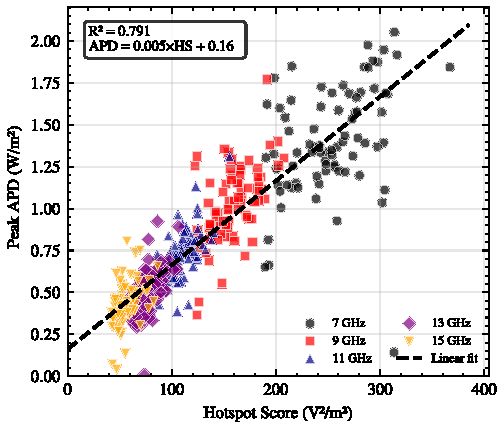
\includegraphics[width=3.5in]{figures/linear_model_sapd_prediction.pdf}
    \caption{Hotspot score predicts actual APD ($R^2 = 0.79$). Points colored by frequency: 7~GHz candidates (black) cluster at high hotspot score and high APD. 15~GHz candidates (orange) cluster at low values.}
    \label{fig:hotspot_regression}
\end{figure}

The frequency-dependent clustering is evident: 7~GHz candidates (black) occupy the upper-right region with high hotspot scores (200--350~V$^2$/m$^2$) and high APD (1.5--2.0~W/m$^2$). 15~GHz candidates (orange) occupy the lower-left region.
The efficient hotspot score reliably predicts actual APD, confirming that the two-stage screening successfully identifies the candidates with the highest values.

\subsection{Comparison with literature}
\label{sec:literature}

Studies in the literature report the worst single plane-wave configuration.
Table~\ref{table:compliance_fr1} gives the average over the 12 configurations, which is 1.5--1.6 times lower.
We therefore compare with the per-configuration values, listed in Table~\ref{table:literature}.

\citet{bakker2010children} simulate the same four phantoms and the same 12 plane-wave configurations.
They report 145\% (Thelonious) and 121\% (Eartha) of the basic restriction, against 145\% and 122\% in this work.
The four worst-case whole-body \gls{SAR} values differ by at most 2\%.
\citet{uusitupa2010sar} simulate three of the same phantoms and report 154\% for Thelonious.
The three values differ by at most 12\%.
\citet{kuehn2009assessment} find the 6-year-old phantom above the restriction at 100~MHz and above 1450~MHz.
The worst configuration in this work first exceeds it at 1450~MHz.
All of these differences are within the expanded uncertainty of $\pm 12$\% ($k = 2$).

\citet{dimbylow2002fdtd} simulate NORMAN, a different phantom.
Its mass is 73~kg, against 72.6~kg for Duke.
The agreement is within 4\% up to 1450~MHz.
Above 2450~MHz Duke absorbs 14--15\% more.
NORMAN is a 2.077~mm voxel model, under 7 cells per wavelength in muscle at 3~GHz.
Coarse voxels under-resolve the body surface, where absorption is concentrated at these frequencies.

No whole-body \gls{SAR} for a child phantom has been reported above 6~GHz.
For FR3 and FR2 we therefore compare against the closed-form model of \citet{kodera2024wbasar}.
Above 10~GHz the absorption cross section of equation~(\ref{eq:sar_acs}) converges to $\mathrm{ACS}_\mathrm{wb} \approx A_\mathrm{p} T$ to within 5\%.
Here $A_\mathrm{p}$ is the projected area of the body seen from the direction of incidence, and $T$ is the Fresnel power transmission coefficient at the skin surface.
For Thelonious under side illumination $A_\mathrm{p} = 0.132$~m$^2$.
The model gives 3.61~mW/kg at 26~GHz, against 3.57~mW/kg in this work.
The excess over the model falls monotonically from 20\% at 7~GHz to 1\% at 26~GHz, as expected in the geometric-optics limit.
The model omits diffraction into the shadow region.
This contribution decreases as the body becomes electrically larger.

\begin{table}[!t]
\centering
\caption{Comparison with whole-body SAR from the literature: \citet{bakker2010children}, \citet{uusitupa2010sar}, \citet{dimbylow2002fdtd}, and the closed-form model of \citet{kodera2024wbasar}. All values are SAR$_\mathrm{wb}$ in mW/kg for a single plane-wave configuration at 1~W/m$^2$ incident. Ratio is this work divided by the literature value.}
\label{table:literature}
\footnotesize
\setlength{\tabcolsep}{2.5pt}
\begin{tabular}{@{}l ccc ccc @{\hspace{0.5em}} l ccc @{\hspace{0.5em}} r ccc@{}}
\toprule
& \multicolumn{6}{c}{\textbf{Worst case near the 2~GHz peak}} & \multicolumn{4}{c}{\textbf{Duke, front}$^c$} & \multicolumn{4}{c}{\textbf{Thelonious, side}$^d$} \\
\cmidrule(lr){2-7} \cmidrule(lr){8-11} \cmidrule(lr){12-15}
& \multicolumn{3}{c}{Bakker (2010)$^a$} & \multicolumn{3}{c}{Uusitupa (2010)$^b$} & \multicolumn{4}{c}{Dimbylow (2002)} & \multicolumn{4}{c}{Kodera (2024)} \\
\cmidrule(lr){2-4} \cmidrule(lr){5-7} \cmidrule(lr){8-11} \cmidrule(lr){12-15}
\textbf{Phantom} & Theirs & Ours & Ratio & Theirs & Ours & Ratio & \textbf{MHz} & Theirs & Ours & Ratio & \textbf{GHz} & Theirs & Ours & Ratio \\
\midrule
Duke & 6.24 & 6.21 & 1.00 & 6.16 & 5.77 & 0.94 & 400 (450) & 6.29 & 6.34 & 1.01 & 7 & 3.29 & 3.96 & 1.20 \\
Ella & 6.76 & 6.60 & 0.98 & 7.53 & 6.60 & 0.88 & 900 (835) & 6.40 & 6.45 & 1.01 & 11 & 3.34 & 3.88 & 1.16 \\
Eartha & 9.68 & 9.76 & 1.01 & -- & -- & -- & 1400 (1450) & 6.33 & 6.11 & 0.96 & 15 & 3.40 & 3.85 & 1.13 \\
Thelonious & 11.60 & 11.61 & 1.00 & 12.32 & 11.61 & 0.94 & 2450 & 4.75 & 5.48 & 1.15 & 26 & 3.61 & 3.57 & 0.99 \\
& & & & & &  & 3000 (3500) & 3.99 & 4.55 & 1.14 & & & &  \\
\bottomrule
\end{tabular}
\par\vspace{3pt}
\begin{minipage}{\textwidth}
\footnotesize $^a$Eartha and Thelonious from their text, Duke and Ella from their figure~4 with the corrigendum applied. $^b$Sampled at 2100~MHz, at the polarization they report: vertical for Duke and Thelonious, horizontal for Ella. Our value is the maximum over our directions at the same polarization. Their VF Male, VF Female and VF Boy are the same subjects as Duke, Ella and Thelonious. They do not include Eartha. $^c$NORMAN, 73~kg against 72.6~kg for Duke. Our frequency in parentheses where it differs. $^d$Closed-form model $\mathrm{ACS}_\mathrm{wb} \approx A_\mathrm{p} T$, with $A_\mathrm{p} = 0.132$~m$^2$ the lateral projected area of Thelonious and $T$ the Fresnel power transmission coefficient of skin.
\end{minipage}
\end{table}

\section{Conclusion}
\label{sec:conclusion}

We characterized \gls{RF}--\gls{EMF} exposure from 450~MHz to 26~GHz using 550 \gls{FDTD} simulations across four phantoms, two exposure scenarios, and 15 frequencies.
Environmental whole-body \gls{SAR} exceeds the basic restriction for both child phantoms near 2140~MHz, in four of the twelve plane-wave configurations.
The adult phantoms stay below the restriction in every configuration.
Under beamforming, basic restrictions are exceeded when the reference levels are met at 3500~MHz (psSAR$_{10\mathrm{g}}$: 131--158\% of the head/torso limit for all four phantoms) and at 7~GHz (APD: 103\% for a 6-year-old).
At 700~MHz, beamforming doubles psSAR$_{10\mathrm{g}}$ with all phantoms remaining within limits.
SAR$_\mathrm{wb}$ remains unchanged. Coherent focusing redistributes absorption spatially without increasing total absorbed power.
At 15~GHz, compliance margins widen to 25--40\% of the basic restriction.
These results indicate that \gls{ICNIRP} reference levels at 3500~MHz and 7~GHz do not guarantee compliance with basic restrictions when beamforming concentrates energy on the body.
Reference levels were derived from uniform plane-wave exposure at a fixed incident power density and do not account for this scenario.
The equal-power components combine in phase at the focus point, so local absorption concentrates while the incident power density stays at the reference level.
At 3500~MHz the volumetric 10~g psSAR$_{10\mathrm{g}}$ in the torso exceeds the limit, and at 7~GHz the 4~cm$^2$ surface \gls{APD} exceeds it.
Measured exposure in deployed 5G networks stays three to four orders of magnitude below this reference level~\citep{veludo2025assessing}, so realistic exposure remains well below the basic restrictions.

Children show 1.5--1.9~times higher whole-body \gls{SAR} than adults at all sub-6~GHz frequencies.
Their higher ratio of absorption cross section to body mass (Eq.~\eqref{eq:sar_acs}) explains this difference.
At 2140~MHz, Thelonious reaches 93\% of the 80~mW/kg limit averaged over the 12 configurations, and 145\% in the worst one. This is the tightest FR1 margin.
Whole-body \gls{SAR} determines FR1 compliance margins. psSAR$_{10\mathrm{g}}$ reaches only 45\% of its limit when whole-body \gls{SAR} reaches 93\%, and stays below its applicable restriction in every environmental configuration.
Worst-case whole-body \gls{SAR} agrees with the literature within 2\% for the same four phantoms, and with a closed-form absorption-cross-section model within 1\% at 26~GHz.

Penetration depth determines tissue-specific absorption.
Lower frequencies lead to higher absorption in deep tissues.
Brain \gls{SAR} decreases 96\% from 450~MHz to 5.8~GHz. Skin \gls{SAR} increases 3.2-fold as $\delta_{90}$ drops from $\sim$60~mm to $\sim$10~mm.
Skin and brain \gls{SAR} correlate negatively ($r = -0.45$, $p < 0.001$) because superficial absorption shields deep tissues such as the brain.

Four phantoms limit inter-individual variability assessment.
More child models (ages 1--17) would strengthen child-adult comparisons.
The 26~GHz analysis includes only Thelonious from one direction due to computational constraints.
Auto-induced simulations use simplified \gls{MRT} beamforming from four directions, not environment-specific channel statistics.
Actual exposure depends on propagation conditions, antenna count, and scattering richness.
All phantoms were simulated in standing configuration. Seated and prone positions may differ in absorption levels.

The organ-specific \gls{SAR} data for brain, eyes, skin, and genitals support epidemiological exposure assessment across 15 frequencies.
The 7.125--8.4~GHz band is on the WRC-27 agenda.
Compliance assessment at this band should include child phantoms.

Several extensions merit investigation.
Posture variations (seated, prone, moving) would quantify how absorption differs from the standing configuration used here.
Coupling this framework with realistic propagation channels~\citep{shikhantsov2020massive,wydaeghe2022realistic,wydaeghe2025outdoor} would quantify how exposure scales with multipath components and antenna elements across environments. This would extend the results beyond the simplified equal-gain scenario used here.
Full characterization of FR2 (24--52.6~GHz) and beyond across all phantoms would complete the 5G and 6G spectrum coverage. As whole-body FDTD simulations become infeasible, other techniques such as those based on the absorption cross section should be used~\cite{kodera2024wbasar}.
Comparison with temperature-rise measurements or \emph{in vivo} exposure data would validate the computational predictions and strengthen the link between dosimetric quantities and biological outcomes.

\funding{The GOLIAT project has received funding from the European Union's Horizon Europe research and innovation programme under grant agreement No.~101057262. Views and opinions expressed are however those of the authors only and do not necessarily reflect those of the European Union or the European Health and Digital Executive Agency. Neither the European Union nor the granting authority can be held responsible for them.}

\roles{R.~Wydaeghe: Conceptualization, Methodology, Software, Validation, Formal analysis, Investigation, Data curation, Writing -- Original Draft, Visualization. B.~Stroobandt: Writing -- Review \& Editing. G.~Vermeeren: Writing -- Review \& Editing. E.~Tanghe: Writing -- Review \& Editing. W.~Joseph: Conceptualization, Supervision, Project administration, Funding acquisition, Writing -- Review \& Editing. S.~Gallucci, M.~Parazzini, G.~Tognola, J.~Wiart, M.~Guxens: Conceptualization, Writing -- Review \& Editing, Funding acquisition.}

\data{The code to produce all the results is available on GitHub at \url{https://github.com/rwydaegh/goliat}. The FDTD simulation configuration files and post-processed SAR/APD datasets supporting this study are available in Harvard Dataverse. The Virtual Population phantoms are available from the IT'IS Foundation under license. The software to produce the results is given in the Supplementary Information and requires licenses for the Sim4Life software from Zurich MedTech AG.}

\suppdata{Supplementary Information contains data, configuration and logging files, as well as 614 figures showing per-tissue SAR values for each frequency and direction, frequency response curves for individual organs, spatial hotspot maps, and cross-phantom comparisons.}

\conflict{The authors declare no conflicts of interest.}

\begin{thebibliography}{99}

\bibitem[Bakker \emph{et al}(2010)]{bakker2010children}
Bakker J F, Paulides M M, Christ A, Kuster N and van Rhoon G C 2010 Assessment of induced SAR in children exposed to electromagnetic plane waves between 10~MHz and 5.6~GHz \emph{Phys. Med. Biol.} \textbf{55} 3115--30

\bibitem[Birks \emph{et al}(2021)]{birks2021dose}
Birks L E, van Wel L, Liorni I, Pierotti L, Guxens M, Huss A, Foerster M, Capstick M, Eeftens M, El Marroun H, Estarlich M, Gallastegi M, Gonz\'{a}lez Safont L, Joseph W, Santa-Marina L, Thielens A, Torrent M, Vrijkotte T, Wiart J, R\"{o}\"{o}sli M, Cardis E, Vermeulen R and Vrijheid M 2021 Radiofrequency electromagnetic fields from mobile communication: description of modeled dose in brain regions and the body in European children and adolescents \emph{Environ. Res.} \textbf{193} 110505

\bibitem[Bamba \emph{et al}(2015)]{bamba2015absorption}
Bamba A, Gaillot D P, Tanghe E, Vermeeren G, Joseph W, Lienard M and Martens L 2015 Assessing whole-body absorption cross section for diffuse exposure from reverberation chamber measurements \emph{IEEE Trans. Electromagn. Compat.} \textbf{57} 27--34

\bibitem[Bj{\"o}rnson \emph{et al}(2017)]{bjornson2017massive}
Bj{\"o}rnson E, Hoydis J and Sanguinetti L 2017 Massive MIMO Networks: Spectral, Energy, and Hardware Efficiency \emph{Found. Trends Signal Process.} \textbf{11} 154--655

\bibitem[Courant \emph{et al}(1928)]{courant1928}
Courant R, Friedrichs K and Lewy H 1928 {\"U}ber die partiellen Differenzengleichungen der mathematischen Physik \emph{Math. Ann.} \textbf{100} 32--74

\bibitem[Dimbylow(2002)]{dimbylow2002fdtd}
Dimbylow P J 2002 Fine resolution calculations of SAR in the human body for frequencies up to 3~GHz \emph{Phys. Med. Biol.} \textbf{47} 2835--46


\bibitem[GOLIAT~Consortium(2022)]{goliat2023}
GOLIAT Consortium 2022 5G expOsure, causaL effects, and rIsk perception through citizen engAgemenT Horizon Europe Project No.~101057262 (available at: \url{https://projectgoliat.eu/})

\bibitem[Gosselin \emph{et al}(2014)]{gosselin2014development}
Gosselin M-C, Neufeld E, Moser H, Huber E, Farcito S, Gerber L, Jedensj{\"o} M, Hilber I, Di~Gennaro F, Lloyd B, Cherubini E, Szczerba D, Kainz W and Kuster N 2014 Development of a new generation of high-resolution anatomical models for medical device evaluation: The Virtual Population 3.0 \emph{Phys. Med. Biol.} \textbf{59} 5287--303

\bibitem[GSMA(2024)]{gsma2024wrc}
GSMA 2024 WRC-23 and WRC-27 -- Mobile Spectrum (available at: \url{https://www.gsma.com/connectivity-for-good/spectrum/wrc-series/})

\bibitem[Hand(2008)]{hand2008modeling}
Hand J W 2008 Modelling the interaction of electromagnetic fields (10~MHz--10~GHz) with the human body: methods and applications \emph{Phys. Med. Biol.} \textbf{53} R243--86

\bibitem[Herssens and Thielens(2025)]{herssens2025autoinduced}
Herssens H and Thielens A 2025 Auto-induced downlink radiofrequency electromagnetic field exposure at 3.5~GHz with focusing near the head \emph{IEEE Access} \textbf{13} 56659--70

\bibitem[Hirata \emph{et al}(2021a)]{hirata2021assessment}
Hirata A \emph{et al} 2021a Assessment of human exposure to electromagnetic fields: Review and future directions \emph{IEEE Trans. Electromagn. Compat.} \textbf{63} 1619--30

\bibitem[Hirata \emph{et al}(2021b)]{hirata2021review}
Hirata A, Kodera S, Sasaki K, Gomez-Tames J, Laakso I, Wood A, Watanabe S and Foster K R 2021b Human exposure to radiofrequency energy above 6~GHz: review of computational dosimetry studies \emph{Phys. Med. Biol.} \textbf{66} 08TR01

\bibitem[ICNIRP(2020)]{icnirp2020}
ICNIRP 2020 Guidelines for limiting exposure to electromagnetic fields (100 kHz to 300 GHz) \emph{Health Phys.} \textbf{118} 483--524

\bibitem[IEC/IEEE(2017)]{iec62704}
IEC/IEEE 2017 62704-1:2017 Determining the peak spatial-average specific absorption rate (SAR) in the human body from wireless communications devices, 30 MHz--6 GHz -- Part 1: General requirements for using the finite-difference time-domain (FDTD) method

\bibitem[IEC/IEEE(2022)]{iec63195}
IEC/IEEE 2022 63195-2:2022 (IEC/IEEE 63195-4) Assessment of power density of human exposure to radio frequency fields from wireless devices in close proximity to the head and body (frequency range of 6~GHz to 300~GHz) -- Part 2: Computational procedure (available at: \url{https://doi.org/10.1109/ieeestd.2022.9770556})

\bibitem[IT'IS~Foundation(2024)]{itis_database}
IT'IS Foundation 2024 Tissue Properties Database V5.0 (available at: \url{https://itis.swiss/virtual-population/tissue-properties/database/})


\bibitem[Kodera \emph{et al}(2024)]{kodera2024wbasar}
Kodera S, Taguchi K, Diao Y, Kashiwa T and Hirata A 2024 Computation of whole-body average SAR in realistic human models from 1 to 100~GHz \emph{IEEE Trans. Microw. Theory Techn.} \textbf{72} 91--100

\bibitem[K{\"u}hn \emph{et al}(2009)]{kuehn2009assessment}
K{\"u}hn S, Jennings W, Christ A and Kuster N 2009 Assessment of induced radio-frequency electromagnetic fields in various anatomical human body models \emph{Phys. Med. Biol.} \textbf{54} 875--90

\bibitem[Liorni \emph{et al}(2020)]{liorni2020evaluation}
Liorni I, Capstick M, van Wel L, Wiart J, Joseph W, Cardis E, Guxens M, Vermeulen R and Thielens A 2020 Evaluation of specific absorption rate in the far-field, near-to-far field and near-field regions for integrative radiofrequency exposure assessment \emph{Radiat. Prot. Dosimetry} \textbf{190} 459--72

\bibitem[Loji\'{c}~Kapetanovi\'{c} and Poljak(2022)]{lojic2022spherical}
Loji\'{c} Kapetanovi\'{c} A and Poljak D 2022 Assessment of incident power density on spherical head model up to 100~GHz \emph{IEEE Trans. Electromagn. Compat.} \textbf{64} 1296--303

\bibitem[Loji\'{c}~Kapetanovi\'{c} \emph{et al}(2023)]{lojic2023ear}
Loji\'{c} Kapetanovi\'{c} A, Sacco G, Poljak D and Zhadobov M 2023 Area-averaged transmitted and absorbed power density on a realistic ear model \emph{IEEE J. Electromagn. RF Microw. Med. Biol.} \textbf{7} 39--45

\bibitem[Marzetta \emph{et al}(2016)]{marzetta2016fundamentals}
Marzetta T L, Larsson E G, Yang H and Ngo H Q 2016 \emph{Fundamentals of Massive MIMO} (Cambridge: Cambridge University Press)

\bibitem[Nakae \emph{et al}(2020)]{nakae2020skin}
Nakae T, Funahashi D, Higashiyama J, Onishi T and Hirata A 2020 Skin temperature elevation for incident power densities from dipole arrays at 28~GHz \emph{IEEE Access} \textbf{8} 26863--71

\bibitem[Next~G~Alliance(2023)]{nextg2023terminology}
Next~G~Alliance 2023 Terminology for Frequency Ranges White Paper (available at: \url{https://nextgalliance.org/white_papers/terminology-for-frequency-ranges/})

\bibitem[Peyman \emph{et al}(2009)]{peyman2009dielectric}
Peyman A, Gabriel C, Grant E H, Vermeeren G and Martens L 2009 Variation of the dielectric properties of tissues with age: The effect on the values of SAR in children when exposed to walkie-talkie devices \emph{Phys. Med. Biol.} \textbf{54} 227--41

\bibitem[Rappaport \emph{et al}(2019)]{rappaport2019wireless}
Rappaport T S, Xing Y, Kanhere O, Ju S, Madanayake A, Mandal S, Alkhateeb A and Trichopoulos G C 2019 Wireless communications and applications above 100~GHz: Opportunities and challenges for 6G and beyond \emph{IEEE Access} \textbf{7} 78729--57

\bibitem[Shikhantsov \emph{et al}(2020)]{shikhantsov2020massive}
Shikhantsov S, Thielens A, Vermeeren G, Demeester P, Martens L, Torfs G and Joseph W 2020 Massive MIMO propagation modeling with user-induced coupling effects using ray-tracing and FDTD \emph{IEEE J. Sel. Areas Commun.} \textbf{38} 1955--63

\bibitem[Katwe \emph{et al}(2024)]{tataria2024cmwave}
Katwe M V, Kaushik A, Singh K, Di~Renzo M, Sun S, Lee D, Armada A G, Eldar Y C, Dobre O A and Rappaport T S 2024 CmWave and Sub-THz: Key Radio Enablers and Complementary Spectrum for 6G \emph{IEEE Wireless Commun.} \textbf{32} 182--90

\bibitem[Taflove and Hagness(2005)]{taflove2005computational}
Taflove A and Hagness S C 2005 \emph{Computational Electrodynamics: The Finite-Difference Time-Domain Method} 3rd edn (Boston, MA: Artech House)

\bibitem[Uusitupa \emph{et al}(2010)]{uusitupa2010sar}
Uusitupa T, Laakso I, Ilvonen S and Nikoskinen K 2010 SAR variation study from 300 to 5000~MHz for 15 voxel models including different postures \emph{Phys. Med. Biol.} \textbf{55} 1157--76

\bibitem[van Wel \emph{et al}(2021)]{vanwel2021organ}
van Wel L, Liorni I, Huss A, Thielens A, Wiart J, Joseph W, R\"{o}\"{o}sli M, Foerster M, Massardier-Pilonchery A, Capstick M, Cardis E and Vermeulen R 2021 Radio-frequency electromagnetic field exposure and contribution of sources in the general population: an organ-specific integrative exposure assessment \emph{J. Expo. Sci. Environ. Epidemiol.} \textbf{31} 999--1007

\bibitem[Velghe \emph{et al}(2021)]{velghe2021protocol}
Velghe M, Aerts S, Martens L, Joseph W and Thielens A 2021 Protocol for personal RF-EMF exposure measurement studies in 5th generation telecommunication networks \emph{Environ. Health} \textbf{20} 36

\bibitem[Veludo \emph{et al}(2025)]{veludo2025assessing}
Veludo A F, Stroobandt B, Van Bladel H, Sandoval-Diez N, Deprez K, Aerts S, Ben Chikha W, Wiart J, Vecsei Z, Necz P P, Thur\'{o}czy G, Benini M, Bonato M, Gallucci S, Tognola G, Parazzini M, Bel\'{a}\v{c}kov\'{a} L, Vaupoti\v{c} N, Mamrot P, Marianska M, Politanski P, Polanska K, Stamets M, de Llobet P, Casta\~{n}o-Vinyals G, Guxens M, Hulls P M, de Vocht F, Joseph W and R\"{o}\"{o}sli M 2025 Assessing radiofrequency electromagnetic field exposure in multiple microenvironments across ten European countries with a focus on 5G \emph{Environ. Int.} \textbf{200} 109540

\bibitem[Vermeeren \emph{et al}(2008a)]{vermeeren2008electronics}
Vermeeren G, Joseph W and Martens L 2008a Whole-body SAR in spheroidal adult and child phantoms in realistic exposure environment \emph{Electron. Lett.} \textbf{44} 790--1

\bibitem[Vermeeren \emph{et al}(2008b)]{vermeeren2008sar}
Vermeeren G, Joseph W, Olivier C and Martens L 2008b Statistical multipath exposure of a human in a realistic electromagnetic environment \emph{Health Phys.} \textbf{94} 345--54

\bibitem[Wydaeghe \emph{et al}(2022)]{wydaeghe2022realistic}
Wydaeghe R, Shikhantsov S, Tanghe E, Vermeeren G, Martens L, Demeester P and Joseph W 2022 Realistic human exposure at 3.5~GHz and 28~GHz for distributed and collocated MaMIMO in indoor environments using hybrid ray-tracing and FDTD \emph{IEEE Access} \textbf{10} 130996--131004

\bibitem[Wydaeghe \emph{et al}(2026)]{wydaeghe2025outdoor}
Wydaeghe R, Shikhantsov S, Tanghe E, Vermeeren G, Martens L and Joseph W 2026 Hybrid ray-tracing-QuaDRiGa/FDTD method for realistic human exposure assessment at 28~GHz with 6G CF-MaMIMO in 3D outdoor environments \emph{npj Wireless Commun.} accepted

\bibitem[Yee(1966)]{yee1966numerical}
Yee K S 1966 Numerical solution of initial boundary value problems involving Maxwell's equations in isotropic media \emph{IEEE Trans. Antennas Propag.} \textbf{14} 302--7

\bibitem[ZMT~Zurich~MedTech~AG(2024)]{sim4life}
ZMT Zurich MedTech AG 2024 Sim4Life: Computational Life Sciences Platform (available at: \url{https://sim4life.swiss/})

\end{thebibliography}

\end{document}
